\documentclass{article}

% PACKAGES  ============================================================
\usepackage{lipsum}		% Used to generate dummy-text (\lipsum[1])
\usepackage[margin=2.54cm,includefoot]{geometry}		% Used to control margins
\usepackage{scrextend}	% To be able to use \begin{addmargin}

\usepackage{graphicx} % allows to import images
\usepackage{float}	% allows for control of float positions
\usepackage{tikz} 	% Used to create trees, neural networks, 
\usetikzlibrary{matrix,chains,positioning,decorations.pathreplacing,arrows} % For neural networks

\usepackage{pgfplots}	% to create plots

\usepackage{forest} % Used to create trees

\usepackage{amsmath}	 % to use cases in equations and vectors

\usepackage[hidelinks]{hyperref}	% allows for clickable references

\usepackage[numbers,sort&compress]{natbib} 	% sorts the cites in increasing order automatically when referenced and compresses successive references

\usepackage[utf8]{inputenc}		% Be able to use umlaute

\usepackage[ngerman]{babel}

\usepackage{fancyhdr}	% Used for Header and Footer stuff

\usepackage{xfrac}	% allows for slanted fractions 

\usepackage{pgfplots}	% Used for function-plots

\usepackage{amssymb} % Use commands like \mathbb
\usepackage{amsmath}
\usepackage{mathtools} % be able to use :=

\usepackage{algorithm}		% Wirte pseudocode algorithms
\usepackage{algorithmic}

\usepackage{subfig} % Figures side by side
%\usepackage[table]  % Used for tables

% ============================================================

% HEADER AND FOOTER STUFF ============================================================
\pagestyle{fancy}
\fancyhead{}	% clears header
\fancyfoot{}	% clears footer
\fancyfoot[R]{\thepage}	% sets position right
\renewcommand{\headrulewidth}{0pt}	% removes header line by setting it to zero
\renewcommand{\footrulewidth}{1pt}		% add footer line by setting it to one
% ============================================================

% DEFINE LIST ITEM BULLETS ============================================================
\renewcommand{\labelitemi}{$\bullet$}	% first list item
\renewcommand{\labelitemii}{$\circ$}	% one-indented item
\renewcommand{\labelitemiii}{$\diamond$}	% twice-indented item
% ============================================================

% BE ABLE TO USE ROW AND COLUMN VECTORS INLINE ============================================================
\newcommand{\icol}[1]{% inline column vector
  \left(\begin{smallmatrix}#1\end{smallmatrix}\right)%
}

\newcommand{\irow}[1]{% inline row vector
  \begin{smallmatrix}(#1)\end{smallmatrix}%
}
% ============================================================

% R Commands =================================================
% Be able to reference sections with number
\newcommand{\secref}[1]{\autoref{#1}. \nameref{#1}}
% ============================================================


% TODO: Diese beiden sollten jeweils das \begin{flushleft} erstzen. 
% Jedoch ist der Text dann im Blocksatz, wenn flushleft fehlt...
%Einrücken von Absätzen deaktivieren
\setlength{\parindent}{0pt}
%Zeilenabstand bei Abstätzen
\usepackage{parskip}

\begin{document}

% TITLE PAGE ============================================================
\begin{titlepage}
	
	\begin{center}
	\line(1,0){330} \\
	[2mm]
	\huge{\bfseries Data Science Zusammenfassung} \\
	[2mm]
	\line(1,0){320} \\
	[1,5cm]
	\textsc{\LARGE By Yannis Schmutz} \\
	[0.75cm]
	\textsc{\large todo} \\
	
	\end{center}
	
\end{titlepage}
% ============================================================

% PREFACE STUFF ============================================================
\pagenumbering{roman}		% sets the page numbering to roman for the preface etc.
\section*{Zusammenfassung}	% Adds a section without a number in front
\addcontentsline{toc}{section}{\numberline{}Zusammenfassung}	% adds a section without a number in front to the ToC
\cleardoublepage	% Finishes the current page so that the following page will always be odd.
% ****************************************************************

% TABLE OF CONTENTS ============================================================
\renewcommand{\contentsname}{Inhaltsverzeichnis}	% Rename table of contents to the german version
\tableofcontents		% adds table of contents (this needs to be compiled twice sometimes in order to update)
\thispagestyle{empty}	% removes header & footer on this page
\cleardoublepage	% Finishes the current page so that the following page will always be odd.
% ============================================================

% LIST OF FIGURES ============================================================
%\renewcommand{\listfigurename}{Abbildungsverzeichnis}	% renames list of figures
\listoffigures	% generates a list of figures
\addcontentsline{toc}{section}{Abbildungsverzeichnis}	% Adds list of figures to the ToC
\cleardoublepage
% ============================================================

% LIST OF TABLES ============================================================
%\renewcommand{\listtablename}{Tabellenverzeichnis}
\listoftables
\addcontentsline{toc}{section}{Tabellenverzeichnis}
\cleardoublepage
% ============================================================

% START OF REGULAR CHAPTERS ============================================================
\setcounter{page}{1}		% Sets this page to the first one (and not the table of contents)
\pagenumbering{arabic}	% Sets the page numbering back to arabic

\newpage
\section{Einleitung}
\label{sec:stat}


Dieses Dokument beschreibt diverse Themen im Bereich Data Engineering, Machine Learning und Data Science. Der Fokus liegt auf dem behandeltem Stoff des Moduls DENG2 der Berner Fachhochschule. \\

\textbf{Prüfungsrelevant} sind die folgenden Kapitel:

\begin{itemize}
  \item \secref{sec:weight_based_learning}
  \item \secref{sec:continuous_learning}
  \item \secref{sec:logistic_regression_basics}
\end{itemize}

\newpage
\section{Statistik}
\label{sec:stat}

\subsection{Begriffe}
\begin{flushleft}
Dieses Kapitel bietet eine grobe Übersicht Über einige hilfreiche Begriffe der Statistik.

\subsubsection{Lageparameter}
Lageparameter beschreiben die Lage der Stichprobenelemente im Bezug auf die Messskala.
\linebreak

\textbf{Mittelwert} \\
Auch Durchschnitt (oder mean im Englischen) gennant. In der Wahrscheinlichkeitsrechnung spricht man oft vom Erwartungswert.

$$\bar{x}_{arithm} = \frac{1}{n} \sum_{i=1}^{n} x_i$$
$$E[X] = \sum_{\omega \in \Omega} p(\omega)*X(\omega)$$

\textbf{Median} \\ 
Der Median oder auch Zentralwert genannt, beschreibt den Wert aus der auf-/ absteigend geordneten Stichprobe, der genau in der Mitte liegt.

\begin{equation*}
  \widetilde{x} = \begin{cases}
    x_{\frac{n+1}{2}}, & \text{\textit{n} ungerade}\\
    \frac{1}{2} \left( x_{\frac{n}{2}} + x_{\frac{n}{1}+1} \right), & \text{\textit{n} gerade}.
  \end{cases}
\end{equation*}


\textbf{Quantile} \\
Schwellenwert (engl. percentile) der angibt, dass ein bestimmter prozentualer Wert einer Menge an Werten kleiner ist als das Quantil. 
Das Quantil bei 50\% ist der Median. Weitere spezielle Quantile sind die Quartile, die Quintile, die Dezile und die Perzentile.
\linebreak

\textbf{Modus} \\
Definiert den häufigsten Wert, der in der Stichprobe vorkommt.
\linebreak

\subsubsection{Streuungsparameter}
Streuungsparameter beschreiben die Streuung von Werten einer Stichprobe um einen bestimmten Lageparameter. So ergeben sich je nach gewählten Lageparameter unterschiedliche Berechungsformen. Diese unterscheiden sich in ihrer Beeinflussung durch Ausreisser. So wird beispielsweise der Median tendenziell weniger von einem einzelnen, sehr hohen Ausreisser beeinflusst als der arithmetische Mittelwert.
\linebreak

\textbf{Spannweite} \\
Die Spannweite (eng. range) gibt den Abstand des grössten gegenüber dem kleinsten vorkommenden Wert der Stichprobe an. $R = x_{max} - x_{min}$.
\linebreak
Die Spannweite wird stark durch Ausreisser beeinflusst. Dem kann jedoch durch das alternative Verwenden des \textbf{Interquartilsabstands} (engl. interquartile range) entgegengewirkt werden. Dieser berechnet nämlich die Spannweite zwischen zwei Quantilen. Somit können Ausreisser ignoriert werden.
\linebreak

\textbf{Varianz} \\



\textbf{Korrelation} \\


\textbf{Kovarianz} \\



\textbf{Kausalität} \\

\subsubsection{Daten}
\textbf{NOIR} \\

\begin{itemize}
	\item \textbf{Nominal}
		\begin{itemize}
			\item Meist diskret
			\item Keine Rangordnung
			\item Bspw: Farben, Geschlecht, Ortschaft etc.
		\end{itemize} 
	\item \textbf{Ordinal}
		\begin{itemize}
			\item Meist diskret
			\item Rangordnung
			\item Keine interpretierbare Abstände
			\item Bspw: Schlecht, okay, gut, sehr gut
		\end{itemize} 
	\item \textbf{Interval}
		\begin{itemize}
			\item Meist stetig
			\item Rangordnung
			\item Interpretierbare Abstände
			\item Kein interpretierbarer Nullpunkt
			\item Bspw: Grad Celsius (geht unter Null)
		\end{itemize} 
	\item \textbf{Rational}
		\begin{itemize}
			\item Meist stetig
			\item Rangordnung
			\item Interpretierbare Abstände
			\item Definierter Nullpunkt
			\item Bspw: Grad Kelvin (geht nicht unter 0K)
		\end{itemize} 

\end{itemize}

\end{flushleft}

% ****************************************************************
\newpage
\section{Probabilistik}
\subsection{Bedingte Wahrscheinlichkeit}

Die bedingte Wahrscheinlichkeit ist die Wahrscheinlichkeit des Eintreten eines Ereignisses A unter der Bedingung, dass die Wahrscheinlichkeit für das Eintreten eines Ereignisses B bereits bekannt ist. Man spricht von \dq{A} unter der Bedingung B\dq. Oder auch $P(A|B)$.\\


Sind zwei Ereignisse E, F voneinander \textbf{unabhängig}, so gilt:
$$ P(E \cap F) = P(E)P(F) $$
$$ P(E|F) = P(E)$$

Sind jedoch zwei Ereignisse A, B \textbf{nicht unabhängig} so lautet die Formel für A unter der Bedingung B:
	$$P(A|B) = \frac{P(A \cap B)}{P(B)}$$


Daraus erschliesst sich:
	$$P(A \cap B) = P(A|B)P(B)$$


Das Aufzeichnen eines Wahrscheinlichkeitsbaumes hilft zur Veranschaulichung: \\

\begin{figure}[H]
	\centering
	\label{fig:probability_tree}
	\begin{forest}
	for tree={circle,draw, s sep=3em}
	[ 
	    [$B$,edge label={node[midway,left] {$P(B)$}}
	      [$A \cap B$,edge label={node[midway,left] {$P(A|B)$}} ] 
	      [$\bar{A} \cap B$,edge label={node[midway,right] {$P(\bar{A}|B)$}}] 
	    ]
	    [$\bar{B}$,edge label={node[midway,right] {$P(\bar{B})$}}
	      [$A \cap \bar{B}$, edge label={node[midway,left] {$P(A|\bar{B})$}}] 
	      [$\bar{A} \cap \bar{B}$, edge label={node[midway,right] {$P(\bar{A}| \bar{B})$}}] 
	  ] 
	]
	\end{forest}
	\caption{Wahrscheinlichkeitsbaum}
\end{figure}

\subsubsection{Satz von Bayes}
%Verweis auf Kapitel \pageref{sec:stat}.

Der Satz von Bayes zeigt den Zusammenhang zwischen $P(A|B)$ und $P(B|A)$ auf:

\begin{equation}
\label{eq:bayes_theorem}
	P(A|B) = \frac{P(A \cap B)}{P(B)} = \frac{P(B|A)P(A)}{P(B)}
\end{equation}

Diese Gleichung \ref{eq:bayes_theorem} entsteht, wenn man den Ausdruck $P(A \cap B)$ anhand den umgekehrten Wahrscheinlichkeitsbaums \ref{fig:inv_probability_tree} ausdrückt. 


\begin{figure}[H]
	\centering
	\label{fig:inv_probability_tree}
	\begin{forest}
	for tree={circle,draw, s sep=3em}
	[ 
	    [$A$,edge label={node[midway,left] {$P(A)$}}
	      [$A \cap B$,edge label={node[midway,left] {$P(B|A)$}} ] 
	      [$A \cap \bar{B}$,edge label={node[midway,right] {$P(\bar{B}|A)$}}] 
	    ]
	    [$\bar{A}$,edge label={node[midway,right] {$P(\bar{A})$}}
	      [$\bar{A} \cap B$, edge label={node[midway,left] {$P(B|\bar{A})$}}] 
	      [$\bar{A} \cap \bar{B}$, edge label={node[midway,right] {$P(\bar{B}| \bar{A})$}}] 
	  ] 
	]
	\end{forest}
	\caption{Umgekehrter Wahrscheinlichkeitsbaum}
\end{figure}
% ****************************************************************




% ****************************************************************
\newpage
\section{Feature Scaling}

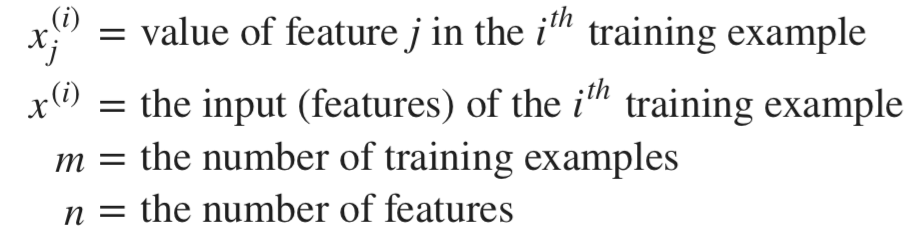
\includegraphics[scale=0.5]{figures/feature_notation}

\subsection{Mean normalization}

$$ x_{j} = \frac{x_{j}^{i} - \mu_{j}}{max(x_{j}) - min(x_{j})} \qquad\forall x^{i} \in x_{j}$$

% ****************************************************************
% ****************************************************************
\newpage
\section{Machine Learning}
\label{sec:ml}

\subsection{Übersicht}

\begin{figure}[H]
	\centering
	\label{fig:ml_overview}
	\begin{forest}
	for tree={draw, s sep=3em}
	[Machine Learning
	    [Überwachtes Lernen
	        [Klassifizierung
	            [Naive Bayes]
	             [k-N-N]
	             [NN]
	        ]
	        [Regression
	            [Linear Regression]
	            [NN]
	        ]
	    ]
	    [Unüberwachtes Lernen
	        [Clustering
	            [K-means]
	        ]
	        [Assoziierung]
	    ]
	]
	\end{forest}
	\caption{Machine Learning Kategorien}
\end{figure}

% #################################
\subsubsection{Überwachtes Lernen}
\begin{flushleft}

Überwachte Lern-Algorithmen probieren Beziehungen und Abhängigkeiten zwischen den Input-Features und des zu erzielenden Outputs zu erschliessen. Dies unter der Verwendung von \textbf{beschrifteten Daten}. Diese können zu Trainingszwecken verwendet werden. Jeder Satz an Daten besteht aus Input-Werten sowie einem dazugehörigen bekannten Output-Wert. Nach dem Trainieren des Algorithmus versucht dieser anhand von \textbf{neuen} Input-Features den dazugehörigen \textbf{unbekannten} Output vorherzusagen.
\linebreak

Das überwachte Lernen kann in zwei Kategorien unterteilt werden:

\begin{itemize}
	\item \textbf{Klassifizierung:} Ziel der Klassifizierung ist es, diskrete Werte vorherzusagen (bspw. Wahr/ Falsch, Spam-Mail/ normales Mail). 
	\item \textbf{Regression:} Das Ziel der Regression ist die Vorhersage kontinuierlicher Werte (bspw. Hauspreise in Abhängigkeit von Flaeche und Anzahl Zimmer).
\end{itemize}

\end{flushleft}

\subsubsection{Unueberwachtes Lernen}
\begin{flushleft}

Im unüberwachten Lernen stehen den Algorithmen \textbf{keine} beschrifteten Daten zur Verfügung. Die Algorithmen versuchen eigenständig Pattern in den zu behandelnden Daten zu erkennen und sie dadurch beispielsweise gruppieren zu können.
\end{flushleft}

% #################################

% ****************************************************************



\newpage
\section{Gewichtbasiertes Lernen}
\label{sec:weight_based_learning}
\subsection{Notationen}
\begin{flushleft}

\begin{align*}
\text{superscript } ^{(i)} &= \text{Index für Samples, Zeilenindex} \\
\text{subscript } _{j} &= \text{Index für Features, Spaltenindex} \\
x^{(i)} &= \text{Die Features des i-ten Samples, Featurevektor} \\
x_{j}^{(i)} &= \text{Der Wert des j-ten Features im i-ten Samples} \\
m &= \text{Die Anzahl Samples} \\
n &= \text{Die Anzahl Features} \\
X &= \text{Datenset} \\
y &= \text{Target Vektor}
\end{align*}

In der Regel ist ein Datenset als Matrix $X$ gegeben mit $\mathbb{R}^{m \times n}$


\begin{center}
	\begin{table}[h]
	\begin{tabular}{|c|c|c|c|c|}
		\hline
		\textbf{Feature 1} & \textbf{Feature 2} & \textbf{...} & \textbf{Feature n} & \textbf{Target} \\ 
		\hline
		$x_{1}^{(1)}$ & $x_{2}^{(1)}$ & ... & $x_{n}^{(1)}$ & Klasse X  \\ 
		\hline
		$x_{1}^{(2)}$ & $x_{2}^{(2)}$ & ... & $x_{n}^{(2)}$ & Klasse Y  \\ 
		\hline
		... & ...  & ... & ...  & ...  \\ 
		\hline
		$x_{1}^{(m)}$ & $x_{2}^{(m)}$  & ... & $x_{n}^{(m)}$  & Klasse Z  \\
		\hline
	\end{tabular}
\end{table}
\end{center}


\end{flushleft}



% === PERCEPTRON ===
\newpage
\subsection{Perceptron}
\begin{flushleft}

                        
Das Perceptron ist ein linearer binärer Klassifikator. In einem Lernprozess generiert das Perceptron eine lineare Funktion, welche Daten in zwei Gruppen unterteilen kann. Eine Gruppe wird oberhalb der Funktionsgeraden liegen, die andere unterhalb.

Eine Konstante (1) wie auch der Feature-Vektor werden individuell mit Gewichten multipliziert und addiert. Ist die Summe grösser als 0, so werden die Input-Features der Klasse 1 zugeordnet. Anderenfalls der Klasse 0.

Für zwei Features $x_{1}$ und $x_{2}$ würde die lineare Funktion wie folgt lauten:
$$w_{0} + x_{1}w_{1} - x_{2}w_{2} = 0$$
                        
                        
\newcommand{\myThresholdFunction}{
\draw[thick] %(-2.25em,0em) -- (1.25em,0em) 
			 (-0.5em,1.25em) -- (-0.5em,-1.25em)
(-0.5em,1.25em) -- (0.5em,1.25em)
(-0.5em,-1.25em) -- (-1.5em,-1.25em)
;}


\begin{figure}[H]
\centering
\label{fig:perceptron}
\begin{tikzpicture}[
     % define styles 
     clear/.style={ 
         draw=none,
         fill=none
     },
     net/.style={
         matrix of nodes,
         nodes={ draw, circle, inner sep=10pt },
         nodes in empty cells,
         column sep=2cm,
         row sep=-9pt
     },
     >=latex
]
% define matrix mat to hold nodes
% using net as default style for cells
\matrix[net] (mat)
{
% Define layer headings
|[clear]| \parbox{1.3cm}{\centering Input\\layer} & 
|[clear]| \parbox{1.3cm}{\centering Gewichtete\\Summe} &
|[clear]| \parbox{1.3cm}{\centering Schwellwert\\Funktion} \\
         
$+1$  		& |[clear]| & |[clear]| \\
|[clear]| 	& |[clear]| & |[clear]| \\
$x_{1}$  	& |[clear]| & |[clear]| \\
|[clear]| 	& $\Sigma$  & \myThresholdFunction \\
\vdots  	& |[clear]| & |[clear]| \\
|[clear]| 	& |[clear]| & |[clear]| \\
$x_{n}$  	& |[clear]| & |[clear]| \\
};
\draw[->] (mat-2-1) -- node[above=1mm] {$w_{0}$} (mat-5-2);
\draw[->] (mat-4-1) -- node[above=1mm] {$w_{1}$} (mat-5-2);
\draw[->] (mat-6-1) -- node[above=1mm] {$\vdots$} (mat-5-2);
\draw[->] (mat-8-1) -- node[above=1mm] {$w_{n}$} (mat-5-2);
\draw[->] (mat-5-2) -- node[above=1mm] {$\hat{y}$} (mat-5-3);
\draw[->] (mat-5-3) -- node[right=2em] {$\begin{cases}
       		1 & \text{wenn } \hat{y} \geq 0, \\
       		0 & \text{sonst.}
    	\end{cases}$} +(2cm,0);
\end{tikzpicture}
\caption{Perceptron als Model}
\end{figure}


Die Entscheidungsfunktion $d$ entscheidet zu welcher Klasse ein gegebener Inputvektor gehört.

\begin{align*}
w_{i}\cdot x &= \hat{y} \\
d(\hat{y}) &= \begin{cases}
       		1 & \text{wenn } \hat{y} \geq 0, \\
       		0 & \text{sonst.}
    	\end{cases} \\
d(w_{i} \cdot x) &= \begin{cases}
       		1 & \text{wenn } \hat{y} \geq 0, \\
       		0 & \text{sonst.}
    	\end{cases} \\
d(w_{i}^{T}x) &= \begin{cases}
       		1 & \text{wenn } \hat{y} \geq 0, \\
       		0 & \text{sonst.}
    	\end{cases} \\
\end{align*}


Im Gegensatz zu vielen anderen gewichtsbasierten Lernalgorithmen werden beim Perceptron die Gewichte \textbf{nur dann aktualisiert, wenn die vorhergesagte Klasse falsch war.}

Definitionen

\begin{align*}
\Delta w_{j}  &= \text{Gewichtsupdate} \\
\hat{y}^{(i)} &= \text{Vorhergesagter (berechneter) Zielwert} \\
y^{(i)} &= \text{Effektiver Zielwert (Label)} \\
\eta &= \text{Learning Rate} \\
(y^{(i)} - \hat{y}^{(i)}) &= \text{Errorfunktion} \\
\end{align*}

Gewichte werden zu Beginn zufällig initialisiert und dann jeweils wie folgt angepasst:
$$w_{j} \coloneqq w_{j} + \Delta w_{j}$$
$$\Delta w_{j} = \eta (y^{(i)} - \hat{y}^{(i)}) x_{j}^{(i)}$$

Im Falle von zwei Input Features, sähe das Aktualisieren der Gewichte so aus:
\begin{align*}
\Delta w_{0} &= \eta (y^{(i)} - \hat{y}^{(i)}) \\
\Delta w_{1} &= \eta (y^{(i)} - \hat{y}^{(i)}) x_{1}^{(i)} \\
\Delta w_{2} &= \eta (y^{(i)} - \hat{y}^{(i)}) x_{2}^{(i)} \\
\end{align*}



% === LERNEN ===
\newpage
\subsubsection{Lernen}
Wir betrachten nun ein Beispiel wie das Perceptron lernt. Die Gewichte werden zufällig wie folgt initialisiert:

\begin{align*}
	 w_{0} &= -0.5\\
	 w_{1} &= 2 \\
	 w_{2} &= -1 \\
\end{align*}

Die Lernrate $\eta$ setzen wir auf $0.5$.
Wir betrachten den Punkt $P_{0} = (3,5)$, welcher der Klasse 0 angehört und berechnen dessen $\hat{y}$.
\begin{align*}
\hat{y} &= w \cdot x \\
		&= -0.5 + 2*3 - 5 \\
		&= 0.5
\end{align*}

Gemäss der Schwellwertfunktion ist der Punkt $P_{0}$ fälschlicherweise der Klasse 1 zugehörig. Daher werden die Gewichte angepasst.

\begin{align*}
\Delta w_{j} &= \eta (y^{(i)} - \hat{y}^{(i)}) x_{j}^{(i)} \\
\Delta w_{0} &= 0.5(0-0.5) \\
			 &= -0.25 \\
\Delta w_{1} &= 0.5(0-0.5)3 \\
			 &= -0.75 \\
\Delta w_{2} &= 0.5(0-0.5)5 \\
			 &= -1.25\\
\end{align*}

Wir passen nun die Gewichte entsprechend an.

\begin{align*}
	 w_{0} &= w_{0} + \Delta w_{0}\\
	 	   &= -0.5 + (-0.25) \\
	 	   &= -0.75 \\
	 w_{1} &= w_{1} + \Delta w_{1} \\
	 	   &= 2 + (-0.75) \\
	 	   &= 1.25 \\
	 w_{2} &= w_{2} + \Delta w_{2} \\
	 	   &= -1 + (-1.25) \\
	 	   &= -2.25 \\
\end{align*}

Diese Grafik zeigt die Perceptron Funktion vor und nach dem ersten Lern-Update. Für den zweiten Punkt (Klasse 1) in der Grafik, würde die Gewichte nicht aktualisiert werden, da dieser bereits korrekt klassifiziert werden würde.


\begin{figure}[H]
	\centering
	\label{fig:perceptron_learning}
	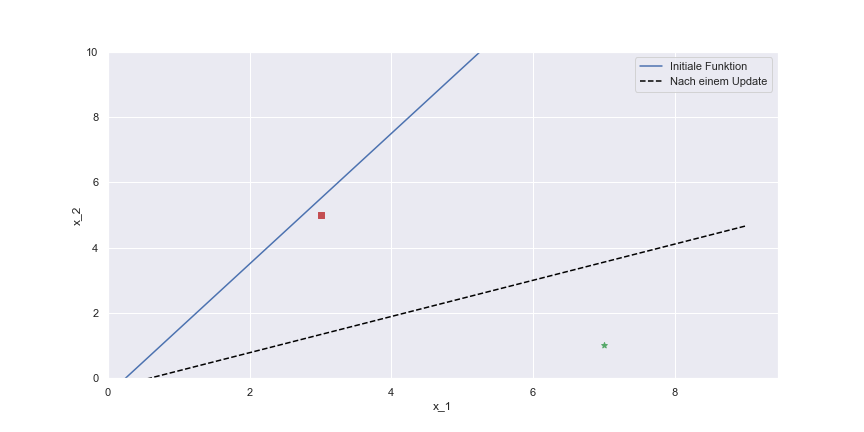
\includegraphics[scale=0.6]{figures/perceptron_learning}
	\caption{Perceptron Lernbeispiel}
\end{figure}




% =======
\newpage
\subsubsection{Vorhersagen}
Im folgenden Beispiel würde sich beispielsweise die Gerade $3x_{1} - x_{2} - 9 = 0$ als Entscheidungsfunktion ergeben. Dies ergibt die Gewichte:
\begin{align*}
	 w_{0} &= -9\\
	 w_{1} &= 3 \\
	 w_{2} &= -1 \\
\end{align*}



Wir betrachten einen Punkt $P_{1} = (5,4)$, eingesetzt in die Entscheidungsfunktion $d$:

\begin{align*}
\hat{y} &= w_{i}\cdot x \\
		&= -9 + 3*5 - 4 \\
		&= 2 \\
d(\hat{y}) &= \begin{cases}
       		1 & \text{wenn } \hat{y} \geq 0, \\
       		0 & \text{sonst.}
       		\end{cases} \\
d(2) &= \text{Klasse 1} \\
\end{align*}

\begin{figure}[H]
	\centering
	\label{fig:perceptron_prediction}
	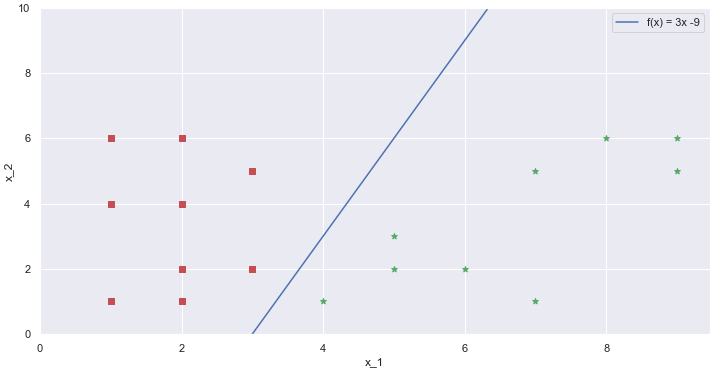
\includegraphics[scale=0.5]{figures/perceptron_line}
	\caption{Perceptron Vorhersage}
\end{figure}

Anhand des Punktes $P_{2} = (2,8)$ zeigen wir, dass das Perceptron auch direkt als Ungleichung angesehen werden kann. Wenn die Ungleichung erfüllt wird, wird der Punkt der Klasse 1 (grüner Stern) zugeordnet. Falls nicht der Klasse 0 (rotes Quadrat)

$$w_{i}\cdot x \geq 0$$
$$ -9 + 3*2 - 8\geq 0$$
$$ -11 \ngeq 0$$

Der Punkt $P_{2}$ wird also der Klasse 0 zugeordnet.

\end{flushleft}

\subsubsection{One-vs-all}
Im One-vs-All (OvA) Verfahren geht es darum mittels eigentlich binären Klassifizierungsverfahren multivariable Klassifizierungen vorzunehmen. Wir wollen also $C > 2$ Klassen unterscheiden können.

Wir wollen also für jede Klasse diese mit den restlichen $C-1$ Klassen unterscheiden können.


\begin{figure}[H]
	\centering
	\label{fig:one_vs_all_vis}
	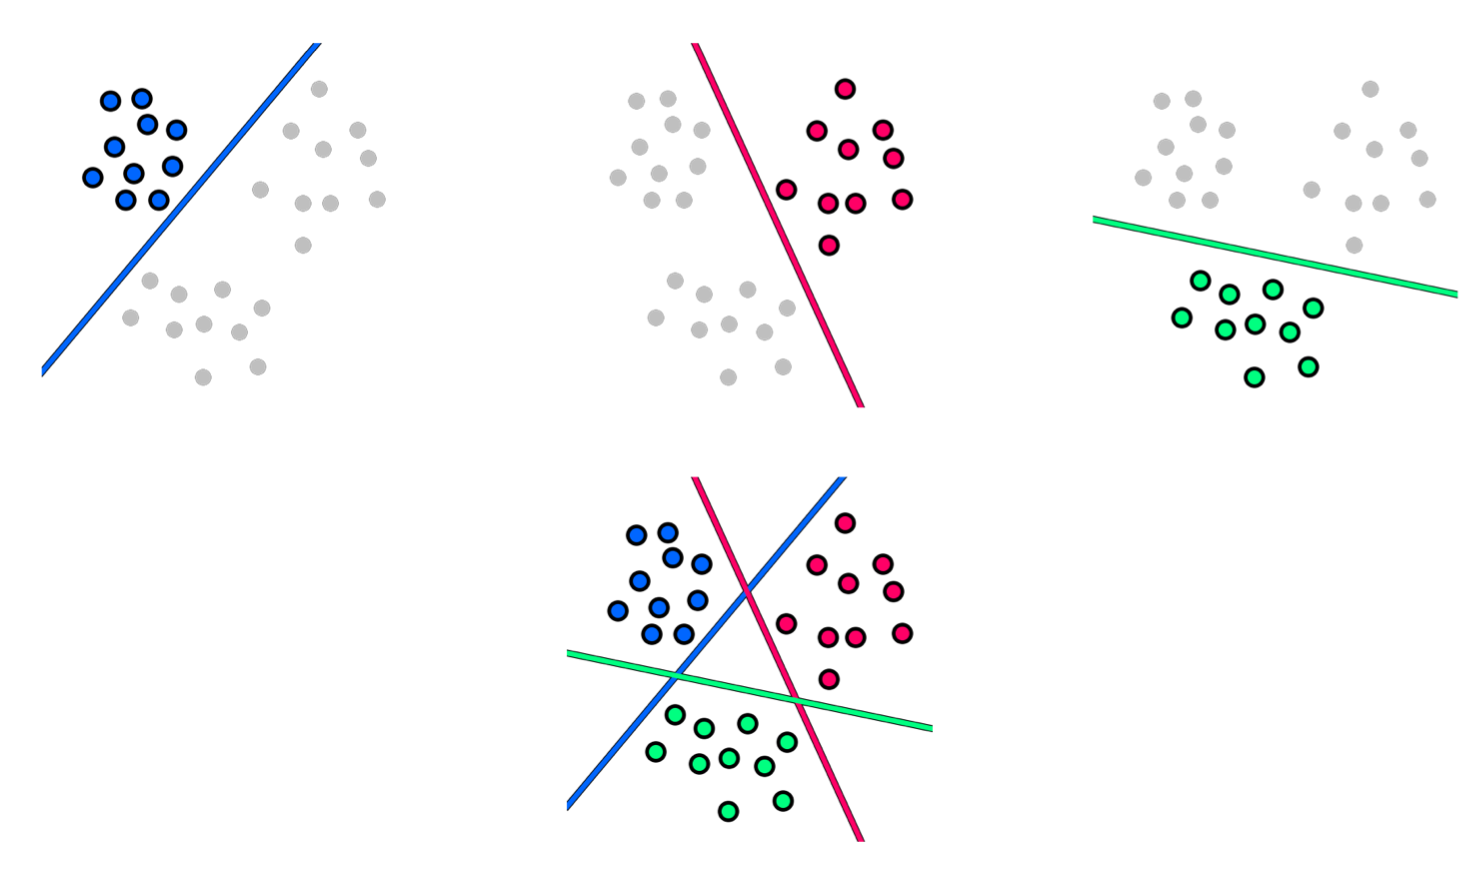
\includegraphics[scale=0.5]{figures/OvA}
	\caption{One-vs-All Visualisierung}
\end{figure}


Angenommen wir haben ein Datenset bestehend aus drei Klassen. Blau, Rot und Grün. Im Datenset ist diesen Klassen jeweils ein numerischen Wert 0, 1 und 2 zugewiesen.


\begin{figure}[H]
	\centering
	\label{fig:one_vs_all_ds_orig}
	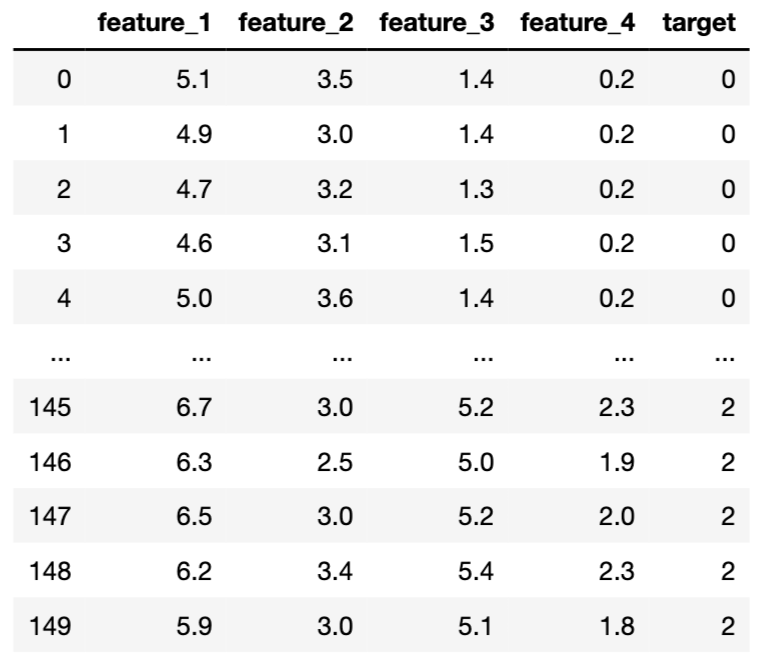
\includegraphics[scale=0.5]{figures/OvA_datenset_original}
	\caption{One-vs-All Datenset original}
\end{figure}


Für das OvA Verfahren werden dem Datenset für jede Klasse eine neue Spalte mit erweiterten temporären Zielvariablen hinzugefügt.

Hierbei wird stets die c-te Klasse betrachtet. In jeder Reihe des Datensets der c-ten Klasse wird ihre temporäre Spalte wird auf $+1$ gesetzt, alle anderen temporären Spalten auf $-1$. 

\begin{figure}[H]
	\centering
	\label{fig:one_vs_all_ds}
	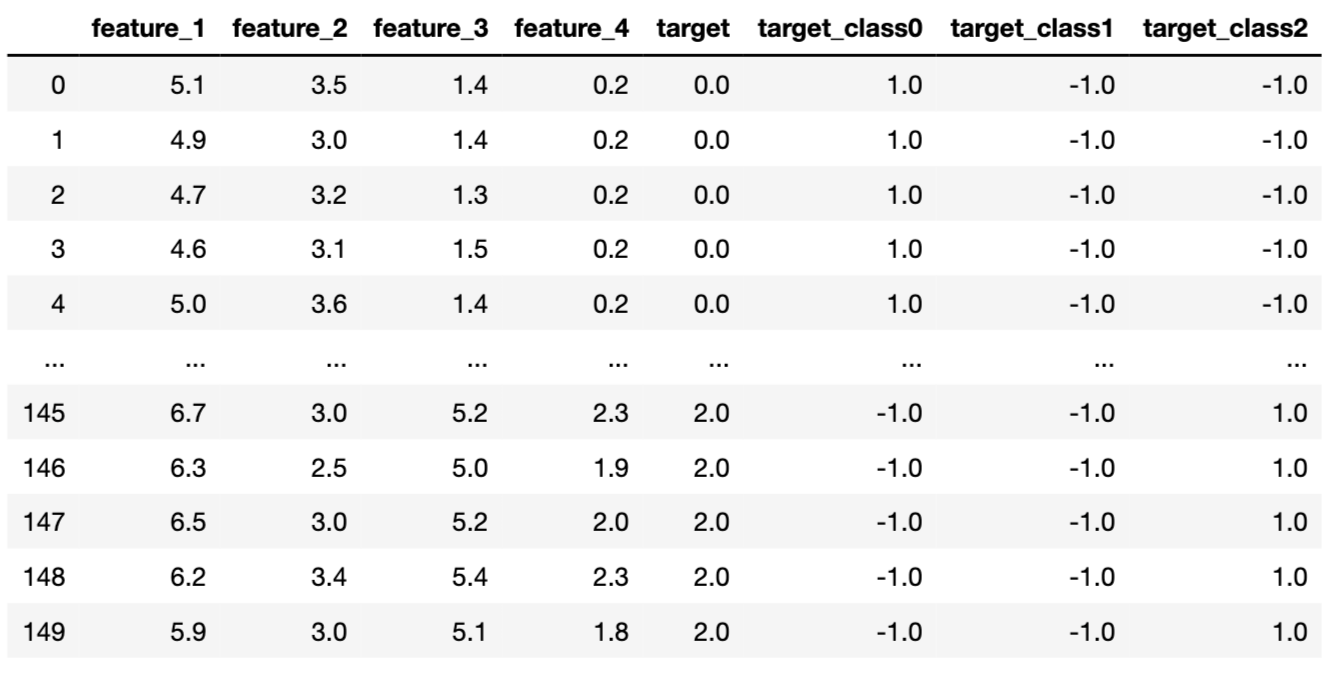
\includegraphics[scale=0.5]{figures/OvA_datenset}
	\caption{One-vs-All Datenset}
\end{figure}


Bisher hatten wir beim Perceptron jeweils ein Gewichtsvektor, welcher eine binäre Unterscheidung durchführt. Nun erhalten wir aber für jede Klasse einen Gewichtsvektor, der sozusagen immer noch eine binäre Unterscheidung durchführt; jedoch zwischen der jeweiligen Klasse und allen anderen Klassen.

In unserem Beispiel haben wir vier Features und drei Klassen. Dies ergibt uns die folgende Gewichtsmatrix.

$W = \begin{bmatrix}
w_{0,0} & w_{0,1} & w_{0,2}\\
w_{1,0} & w_{1,1} & w_{1,2}\\
w_{2,0} & w_{2,1} & w_{2,2}\\
w_{3,0} & w_{3,1} & w_{3,2}\\
w_{4,0} & w_{4,1} & w_{4,2}\\
\end{bmatrix}$


Der erste Index referiert jeweils das entsprechende Feature und der zweite der Index der Klasse.

Ist die Matrix initialisiert, müssen wir für jede Klasse den entsprechenden Gewichtsvektor trainieren. 

Ein zu klassifizierendes Sample wird einer Klasse zugewiesen, indem alle berechneten Outputs der Gewichtsvektoren betrachtet werden. Das Sample wird der Klasse zugeordnet, welche den höchsten Output generiert.

$$ \hat{y} = \text{max}_{c=0,...,C-1} \text{model.predict}(x, W)$$

\newpage
\subsection{Interpretation}
\begin{flushleft}

\subsubsection{Problematik}
\begin{flushleft}

In der klassischen Software-Entwicklung können wir auftretende Bugs mittels Debugging ausfindig machen. Sobald wir den Bug lokalisiert haben beheben wir diesen, indem wir nur einen gewissen Teil unseres Programmes anpassen.

Um uns vor zukünftigen Bugs zu schützen, schreiben wir automatisierte Tests. Diese sollen verifizieren, dass auch bei künftigen Änderungen die bisherigen Features wie gewohnt funktionieren.

Diese "klassischen" Prozesse lassen sich jedoch (momentan) nicht eins zu eins auf einen ML-Workflow anwenden. Damit Machine Learning in Zukunft richtig funktionieren kann, müssen folgende Methoden entwickelt und etabliert werden:


\begin{itemize}
  \item ML Prozesse, Modelle und Integrationen debuggen können.
  \item Entdeckte Bugs beheben können.
  \item Automatisierte Testverfahren, die das Verhalten unserer ML-Lösung verifizieren.
  \item Sicher stellen, dass sich unser Model auch nach einem erneuten Trainieren oder sonstigen Änderungen noch wie erwartet verhält.
\end{itemize}

Um diese Methoden erfolgreich umzusetzen, müssen ML Modelle und Prozesse interpretiert werden können.

\end{flushleft}


\subsubsection{Blackbox}
\begin{flushleft}
Eine grosse Schwierigkeit in der ML Domäne ist, dass Modelle wie auch Probleme oftmals einer Blackbox ähneln.


\end{flushleft}


TODO

\begin{itemize}
  \item Test the effect of $\eta$ (eta) by training with Perceptron versions without it.
  \item Understanding the effect of $\eta$ (eta) and its relation with epochs by identifying bounds for too high or too low $\eta$ values.
  \item Develop a strategy for finding optimal hyperparameters
  \item Peter Norvig's ideas for the future of Machine Learning 
  \item The concept of Interpretability
  \item The concept of Epxlainability
\end{itemize}




\end{flushleft}





\newpage
\section{Continuous Learning}
\label{sec:continuous_learning}

Beim obigen Beispiel (Perceptron) wurde der Error berechnet indem der Vorhersagewert (Klasse, 1 oder 0) vom erwarteten Wert subtrahiert wurde.

In diesem Kapitel werden Ansätze angeschaut, welche auch schauen \textbf{wie weit weg} die Vorhersage war.

\subsection{Adaline}
%\begin{flushleft}

Adaline steht für \textbf{Adaptive Linear Neuron} und ist ein \textbf{supervised classification Algorithmus}. Adaline funktioniert wie folgt:

\begin{itemize}
  \item Die Elemente des Input-Vektors (Featurevektors) werden jeweils mit einem Gewicht multipliziert und aufsummiert.
  \item Die Summe (z) wird einer \textbf{Aktivierungsfunktion} übergeben, welche den Wert $\hat{y}$ erzeugt.
  \item $\hat{y}$ wird dann verwendet, um den \textbf{Fehler} bzw. das \textbf{Update für die Gewichte} zu berechnen.
  \item $\hat{y}$ wird zudem einer \textbf{Schwellwertfunktion} übergeben, welche die Features einer Klasse zuordnet.
\end{itemize}




\newcommand{\myThresholdFunction}{
\draw[thick] %(-2.25em,0em) -- (1.25em,0em) 
			 (-0.5em,1.25em) -- (-0.5em,-1.25em)
(-0.5em,1.25em) -- (0.5em,1.25em)
(-0.5em,-1.25em) -- (-1.5em,-1.25em)
;}


\begin{figure}[H]
\centering
\label{fig:perceptron}
\begin{tikzpicture}[
     % define styles 
     clear/.style={ 
         draw=none,
         fill=none
     },
     net/.style={
         matrix of nodes,
         nodes={ draw, circle, inner sep=10pt },
         nodes in empty cells,
         column sep=1.5cm,
         row sep=-9pt
     },
     >=latex
]
% define matrix mat to hold nodes
% using net as default style for cells
\matrix[net] (mat)
{
% Define layer headings
|[clear]| \parbox{1.3cm}{\centering Input\\layer} & 
|[clear]| \parbox{1.3cm}{\centering Gewichtete\\Summe} &
|[clear]| \parbox{1.3cm}{\centering Aktivierungs\\funktion} &
|[clear]| \parbox{1.3cm}{\centering Schwellwert\\Funktion} \\
         
$+1$  		& |[clear]| & Error     & |[clear]| \\
|[clear]| 	& |[clear]| & |[clear]| & |[clear]| \\
$x_{1}$  	& |[clear]| & |[clear]| & |[clear]| \\
|[clear]| 	& $\Sigma$  & $\phi$ & \myThresholdFunction \\
\vdots  	& |[clear]| & |[clear]| & |[clear]| \\
|[clear]| 	& |[clear]| & |[clear]| & |[clear]| \\
$x_{n}$  	& |[clear]| & |[clear]| & |[clear]| \\
};
\draw[->] (mat-2-1) -- node[above=1mm] {$w_{0}$} (mat-5-2);
\draw[->] (mat-4-1) -- node[above=1mm] {$w_{1}$} (mat-5-2);
\draw[->] (mat-6-1) -- node[above=1mm] {$\vdots$} (mat-5-2);
\draw[->] (mat-8-1) -- node[above=1mm] {$w_{n}$} (mat-5-2);
\draw[->] (mat-5-2) -- node[above=1mm] {$z$} (mat-5-3);
\draw[->] (mat-5-3) -- node[above=1mm] {$\hat{y}$} (mat-5-4);
\draw[->] (mat-5-3) -- node[above=1mm] {$$} (mat-2-3);
\draw[->] (mat-2-3) -- node[above=1mm] {Update Gewichte} (-2.5cm, 1cm);

\draw[->] (mat-5-4) -- node[right=2em] {$\begin{cases}
       		1 & \text{wenn } \hat{y} \geq 0, \\
       		0 & \text{sonst.}
    	\end{cases}$} +(2cm,0);
\end{tikzpicture}
\caption{Adaline als Model}
\label{fig:adaline_model}
\end{figure}


\newpage
Hier eine vereinfachte Beschreibung des Adaline-Models.

\textbf{Training} \\
Füge Bias-Gewicht (1) an Stelle Feature-0 hinzu.
Bestimme $z$:
\begin{align*}
	z &= w^{T} \times x \\
	z &= \sum_{i=0}^{n} w_{i}x_{i}  \\
\end{align*}


Einfachheitshalber nutzen wir für die \textbf{Aktivierungsfunktion} die Identitätsfunktion:
 $$\phi(z) = z$$
 
 Rechne nach jeder \textbf{Epoche} den Error aus und aktualisiere dementsprechend die Gewichte.



\textbf{Prediction} \\
Nun benötigen wir nur noch eine \textbf{Schwellwertfunktion} (decision function), die die vorhergesagte Klasse bestimmt.

$$ d(\hat{y}) =
\begin{cases}
	1 & \text{wenn } \hat{y} \geq 0, \\
	0 & \text{sonst.}
\end{cases}
$$


% ============================================
\newpage
\subsubsection{Adaline vs Perceptron}

Ähnlich wie der Perceptron ist Adaline ein Einzellayer neuronales Netzwerk. Der Hauptunterschied liegt auf der Aktivierungsfunktion phi $\phi(z)$


\begin{itemize}
  \item Der \textbf{Perceptron} aktualisiert die Gewichte nur, wenn eine falsche Vorhersage getroffen wurde. Zudem wird die Error-Funktion erst nach der \textbf{Schwellwertfunktion} aufgerufen. Somit wird ihr stets immer nur eine 0 oder 1 übergeben.
  \item \textbf{Adaline} hingegen aktualisiert die Gewichte basierend auf einer \textbf{stetigen} Funktion (continuous). Der \textbf{Aktivierungsfunktion $\phi$}
 \end{itemize}



Wie in Abbildung \ref{fig:adaline_vs_perceptron} ersichtlich ist, werden die Gewichte bei Adaline \textbf{vor} der Entscheidungsfunktion aktualisiert.

\begin{figure}[h!]
	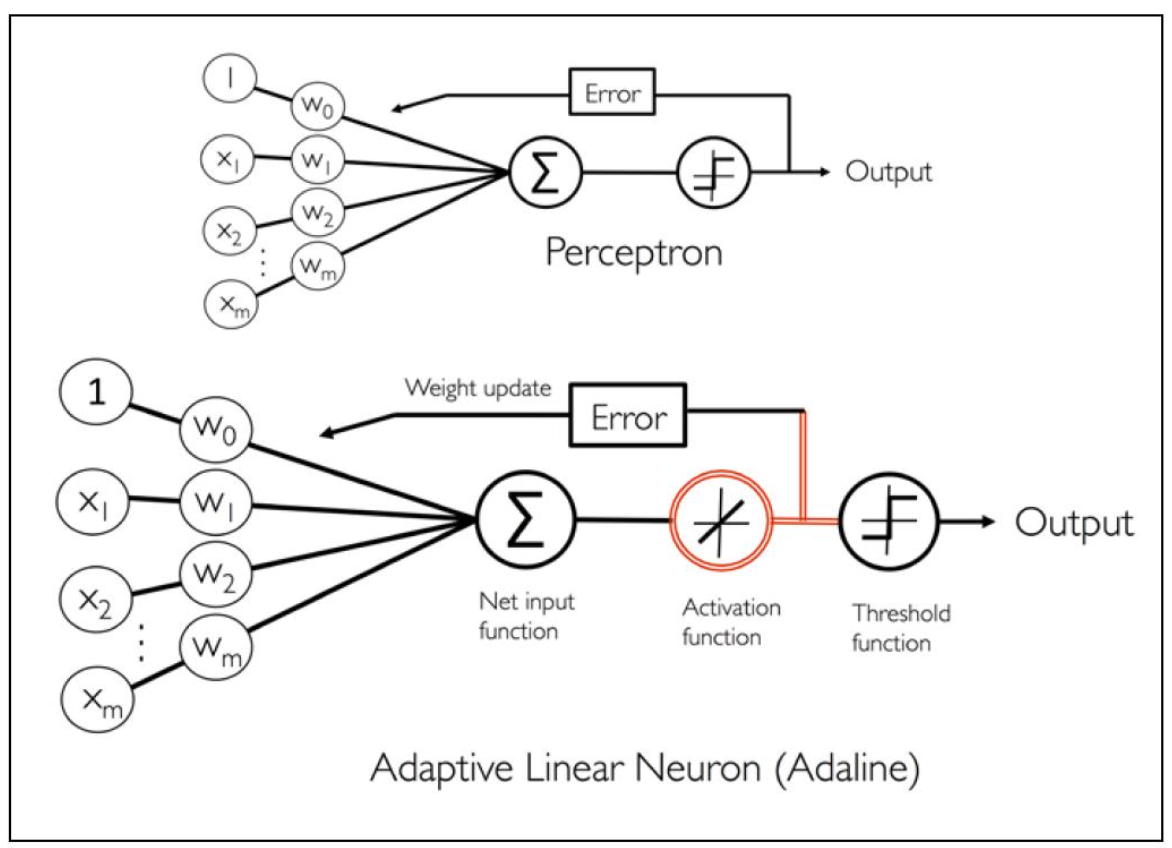
\includegraphics[scale=0.6]{figures/adaline_vs_perceptron}
	\caption{Adaline vs Perceptron}
	\label{fig:adaline_vs_perceptron}
\end{figure}

Im Gegensatz zum \textbf{binären Lernansatz} des Perceptron basieren viele supervised learning Algorithmen auf einer sogenannten \textbf{objective learning function}.


\newpage
\subsubsection{Objective Function}

Die Objective Function (Zielfunktion) ist mathematisch eine \textbf{Optimierung}.

Das Ziel hierbei ist es \textbf{optimale Parameter} zu finden. Optimal bedeutet den Output der Funktion entweder zu \textbf{maximieren} oder zu \textbf{minimieren}. 


Bei Machine Learning entsprechen die Parameter den \textbf{Gewichten}.


Eine Objective Funktion berechnet einen Output basierend auf den Eingaben:

\begin{itemize}
  \item Vorhersage (prediction)
  \item Eigentlicher Wert (labelled value)
\end{itemize}

Hierbei soll deren Differenz möglichst klein werden. Somit ist die Vorhersage sehr nahe am eigentlichen Wert. Ein Beispiel dafür zeigt Abbildung \ref{fig:objective_minimum}. 


\begin{figure}[h!]
	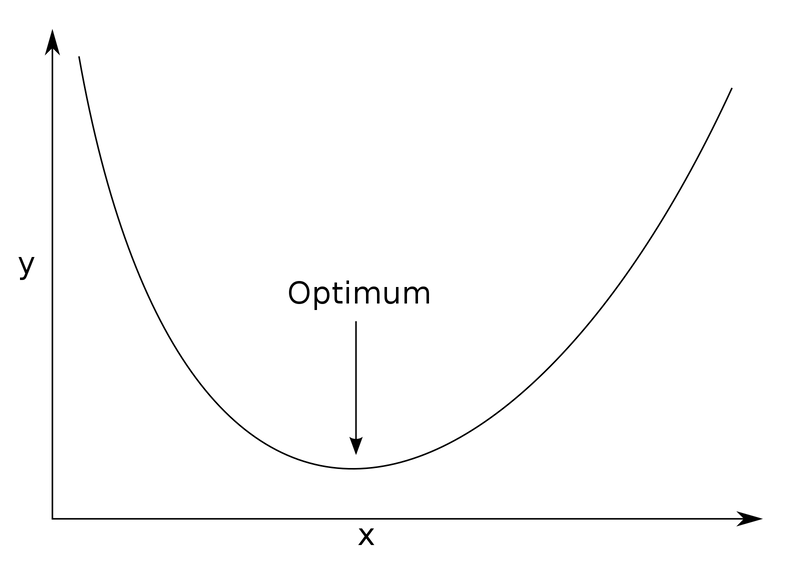
\includegraphics[scale=0.4]{figures/objective_minimum}
	\caption{Beispiel Zielfunktion}
	\label{fig:objective_minimum}
\end{figure}



Objective Funktion ist ein sehr genereller Term im Bereich ML.
Meistens wollen wir den Output der Objective Funktion \textbf{minimieren}. In diesem Fall sprechen wir von einer \textbf{Cost Function} oder \textbf{Loss Function}.


Wollen wir den Output \textbf{maximieren} so sprechen wir von einer \textbf{Likelihood Maximization} Funktion.



 
\newpage
\subsubsection{Objective Function in Adaline}

Adaline verwendet die Cost Function \textbf{Sum of Squared Errors (SSE)}.

SSE summiert alle quadrierten Differenzen zwischen Vorhersage und effektivem Wert auf.

$$ SSE = \frac{1}{2} \sum_{i=1}^{m}(y^{(i)} - \hat{y}^{(i)})^{2} $$

Hier eine detailliertere Darstellung von $\hat{y}$

$$ SSE = \frac{1}{2} \sum_{i=1}^{m}(y^{(i)} - \phi(z^{(i)}))^{2} $$


Wichtig zu wissen:
\begin{itemize}
  \item Die Funktion SSE ist \textbf{differenzierbar (ableitbar)}. Daher kann für jeden Punkt die Steigung berechnet werden.
  \item Sie hat ein \textbf{globales Minimum}.
\end{itemize}


Diese beiden Punkte sind notwendig für \textbf{Optimierungsalgorithmen}. Diese helfen dabei den Wert der Gewichte zu bestimmen damit die Cost Function möglichst klein wird. (Bsp. Gradient Descent)


\subsubsection{Adaline Learning Rule}

Die Gewicht-Updates werden anhand von \textbf{allen Samples} berechnet (Summe von 1 bin m). Daher werden die Gewichte auch immer erst nach einem vollen Trainingsdurchlauf aktualisiert und nicht nach jedem Sample.

Diese Art von Aktualisierung wird \textbf{batch gradient descent} genannt.

\begin{align*}
	\Delta w &= \eta \sum_{i=1}^{m} (y^{(i)} - \phi(z^{(i)}))^{2} * x^{(i)} \\
	w &= w + \Delta w \\
\end{align*}

\begin{align*}
	w &= \text{Gewichtsvektor} \\
	\Delta w &= \text{Gewichtsupdate (Vektor)} \\
	\eta &= \text{Learning Rate} \\
	m &= \text{Anzahl Samples}	\\
	y^{(i)} &= \text{Effektiver Zielwert (Label)} \\
	\phi &= \text{Aktivierungsfunktion} \\
	z^{(i)} &= \text{Summe der Input-Gewicht-Multiplikationen} \\
	x^{(i)} &= \text{Feature-Vektor des Samples i} \\
\end{align*}


\subsubsection{Adaline Optimierung mit Gradient Descent}

Für Adaline kann \textbf{Gradient Descent Algorithmus} zur Justierung verwendet werden.

Die Gewichtsupdates können nun so berechnet werden:

$$ \Delta w = - \eta \nabla J(w) $$

\begin{align*}
	J &= \text{Kostenfunktion (bspw. SSE)} \\
	\nabla &= \text{Symbol für Gradient (Steigung)} \\
	w &= \text{Gewichtsvektor} \\
\end{align*}


Wir berechnen also jeweils die \textbf{Steigung der cost function} am Punkt $P(w, J(w))$.

Der Gradient Descent wird in Kapitel \ref{sec:gradient_descent_basics} genauer erklärt.

% ==================================
\subsection{Gradient Descent Basics}
\label{sec:gradient_descent_basics}

Dieses Kapitel behandelt den Stoff zu Gradient Descent, welcher im Rahmen der Vorlesung behandelt wurde. Vertiefte Informationen zu Gradient descent sind Kapitel \ref{sec:gradient_descent} zu entnehmen.


\begin{itemize}
	\item Die \textbf{optimalen Gewichte} für eine \textbf{objective function} zu finden ist sehr rechenintensiv.
	\item Umso mehr Features vorhanden sind, desto mehr Gewichte hat unser Model.
	\item Daher auch mehr Kombinationen, wie die Gewichte gewählt werden könnten.
\end{itemize}

Optimisierungsalgorithmen (bspw. Gradient Descent) helfen dabei eine effiziente Lösung für die optimalen Gewichte zu finden.


\newpage
\subsubsection{Funktionsweise}

Abbildung \ref{fig:gradient_descent_simple} stellt eine vereinfachte Funktionsweise des GD dar.

\begin{itemize}
	\item Auf der y-Achse sind die Kosten (cost function)
	\item Auf der x-Achse sind die Gewichte. In diesem Beispiel haben wir nur ein Gewicht. Eigentlich wäre die Funktion aber multidimensional.
	\item Der schwarze Punkt zeigt die Ausgangslage bei zufällig initialisierten Gewichten.
	\item Der GD rechnet nun jeweils für die aktuelle Position $P(w, J(w))$ die Steigung aus.
	\item Ist die Steigung positiv müssen wir nach links gehen, um näher ans optimale Minimum zu gelangen. Also das Gewicht reduzieren.
	\item Ist die Steigung negativ, so gehen wir nach rechts indem wir das Gewicht erhöhen.
	\item Die Grösse der Schritte, die wir nach Links oder Rechts gehen wird von der \textbf{learning rate $\eta$} beeinflusst.
\end{itemize}

\begin{figure}[h!]
	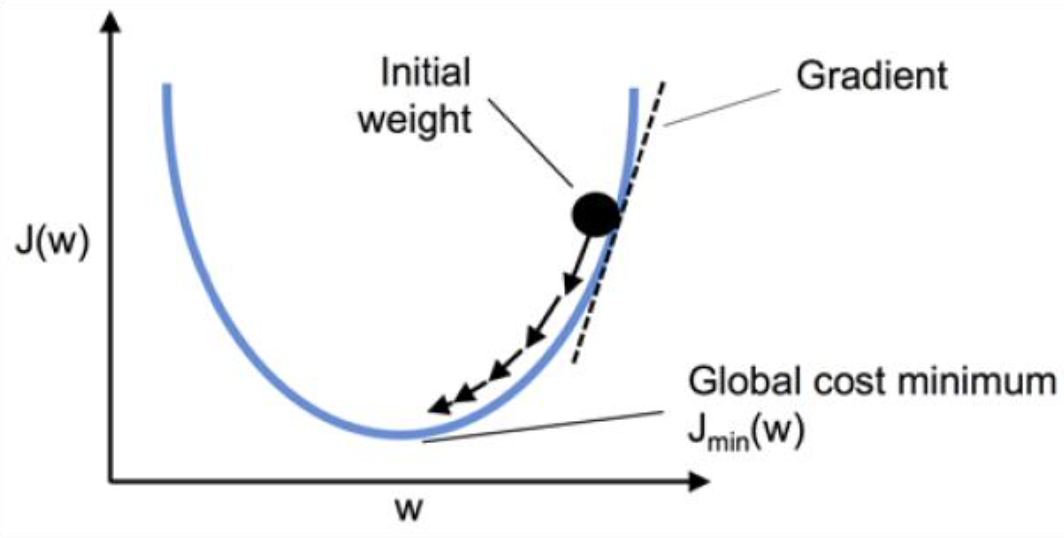
\includegraphics[scale=0.5]{figures/gradient_descent_simple}
	\caption{Gradient Descent Funktionsweise}
	\label{fig:gradient_descent_simple}
\end{figure}

Abbildung \ref{fig:gd_simple_multi} zeigt wie der GD bei mehreren Gewichten aussehen könnte.


\newpage
\subsubsection{Verhalten des GD}

Eine \textbf{optimale cost function ist konvex}. Also wie eine Schüssel geformt. Somit hat die Funktion nur \textbf{ein} Minimum. (Abbildung \ref{fig:gradient_descent_simple})


In der Praxis sehen die Funktionen aber meist wie
bspw. Abbildung \ref{fig:gd_simple_multi} aus. Diese Funktion hat ein \textbf{globales Minimum} und mehrere \textbf{lokale}. Das globale ist der optimale Wert unserer cost function. Doch nicht immer vom GD erreichbar.

\begin{figure}[h!]
	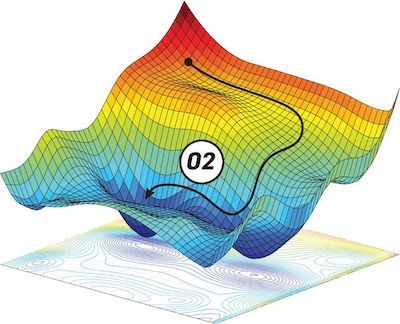
\includegraphics[scale=0.6]{figures/gd_simple_multi}
	\caption{Gradient Descent multidimensional}
	\label{fig:gd_simple_multi}
\end{figure}


\begin{itemize}
	\item Wird die \textbf{learning rate zu hoch} gewählt, ist es möglich, dass der GD stets \textbf{über} dem Minimum rüber springt.
	\item Ist sie \textbf{zu tief}, so könnte der GD in einem \textbf{lokalen Minumum} festsitzen.
\end{itemize}

\begin{figure}
    \centering
    \subfloat[]{{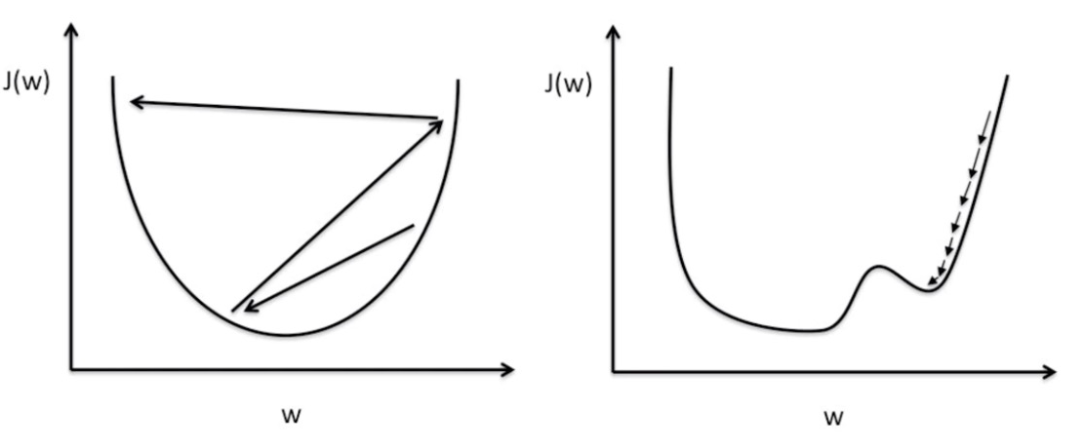
\includegraphics[scale=0.5]{figures/gd_behaviour} }}%
    \qquad
    \subfloat[]{{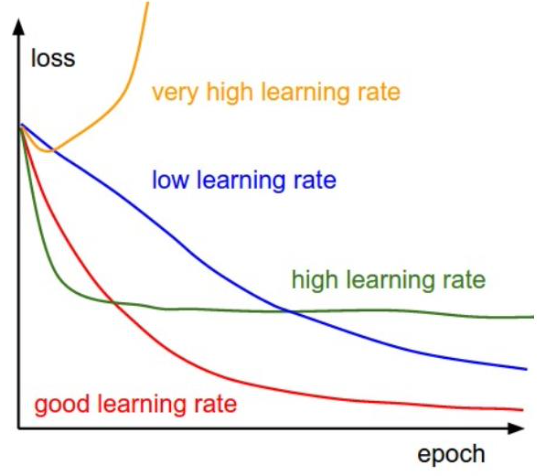
\includegraphics[scale=0.5]{figures/gd_learning_rate} }}%
    \caption{GD learning rate}%
    \label{fig:gd_learning_rate}%
\end{figure}


\newpage
\subsubsection{Arten von GD}

Es gibt verschiedene Möglichkeiten den Gradient Descent zu berechnen.

\textbf{Batch Gradient Descent (BGD)} \\


\begin{itemize}
	\item Verwendet \textbf{alle} Samples der Trainingsdaten \textbf{für eine einzige} Gewichtsaktualisierung.
	\item Für jedes Gewicht (bzw. Feature) wird der Error berechnet, indem der Durchschnittswert über alle Samples verwendet wird.
	\item Outliers haben weniger Einfluss auf die Gewichtsanpassung.
\end{itemize}

Dies führt zu einem stabilen Pfad hin zur Konvergenz gegen das Minimum. \\

Nachteile des BGD:

\begin{itemize}
	\item Schwierig zu \textbf{Skalieren}
	\begin{itemize}
		\item Alle Trainingsdaten (Matrix X) muss in RAM passen.
		\item Pro eine Gewichtsanpassung muss das ganze Trainingset einmal durchlaufen werden. Benötigt viel Epochen.
		\item Heutzutage nicht mehr ganz so tragisch.
	\end{itemize}
	\item Resultierendes Model hat Schwierigkeiten zu \textbf{generalisieren}
	\begin{itemize}
		\item Model leidet oftmals an \textbf{overfitting}
		\item Hauptgrund, um BGD nicht zu verwenden.
	\end{itemize}
\end{itemize}




\textbf{Stochastic Gradient Descent (SGD)} \\

Der stochastischen GD aktualisiert die Gewichte nach \textbf{jedem Schritt (nach jedem einzelnen Sample)}. Dies ist hilfreich für \textbf{grössere Mengen an Trainingsdaten}, da weniger Epochen ausgeführt werden müssen. SGD ist also 

\begin{itemize}
	\item Ist effizienter zu \textbf{Skalieren}
	\item Kleinere Tendenz für \textbf{overfitting} im Vergleich zu BGD.
\end{itemize}


Die Gewichte werden nach jedem Schritt wie folgt berechnet:
$$ w = w - \eta \nabla_{w} J(x^{(i)}, y^{(i)}, w) $$


Nachteile des SGD:

\begin{itemize}
	\item Benötigt viele Trainingsschritte
	\item Ausreisser können den SGD in eine falsche Richtung führen.
\end{itemize}


\newpage
\textbf{Mini-Batch Gradient Descent (MBGD)} \\

Wird oft verwendet. Ist ein \textbf{Kompromiss} zwischen BGD und SGD.
Das Gewichtsupdate wird anhand von $b$ vielen Samples berechnet.

$$ w = w - \eta \nabla_{w} J(x^{(i:i+b)}, y^{(i:i+b)}, w) $$ \\


\begin{itemize}
	\item Hilft \textbf{Overfitting / generalization error} zu vermeiden
	\begin{itemize}
		\item Die Batchgrösse $b$ muss wesentlich kleiner sein als die Anzahl Samples $m$.
		\item Dadurch wird dem Lernprozess \textbf{Noise} beigefügt.
	\end{itemize}
	\item Ist \textbf{schneller} als SGD
	\begin{itemize}
		\item Berechnungen erfolgen auf einer Matrix und nicht auf einzelnen Werten.
		\item Dies erlaubt effiziente Berechnungen mittels \textbf{Vektorisierung}.
	\end{itemize}
\end{itemize}


\textbf{Weitere Varianten} \\

\begin{itemize}
	\item AdaGrand (Adaptive Gradient Descent)
	\begin{itemize}
		\item Verschiedene learning rates für jedes Feature
		\item Nicht alle Features haben die gleichen \textbf{Seltenheit} (sparsity) und Werteverteilungen.
		\item Eine höhere learning rate für seltene (sparse) Features steigert deren Beitrag.
		\item Gut geeignet für NLP.
	\end{itemize}
	\item RMSprop
	\begin{itemize}
		\item Learning rate nimmt im Verlauf der Zeit ab.
		\item Umso kleiner die Steigung wird, desto kleiner wird die learning rate.
	\end{itemize}
\end{itemize}






% ****************************************************************
\newpage
\section{Gradient Descent}
\label{sec:gradient_descent}

\begin{flushleft}

Gradient Descent ist ein Optimierungsalgorithmus, um ein lokales Minimum einer Funktion zu finden.
Gegeben sei eine Kosten-Funktion $J(\Theta_{0}, \Theta_{1})$, gesucht ist das Minimum der Funktion $min_{\Theta_{0}, \Theta_{1}} J(\Theta_{0}, \Theta_{1})$, indem die Parameter $\Theta_{0}$ und $\Theta_{0}$ laufend ein wenig verändert werden.

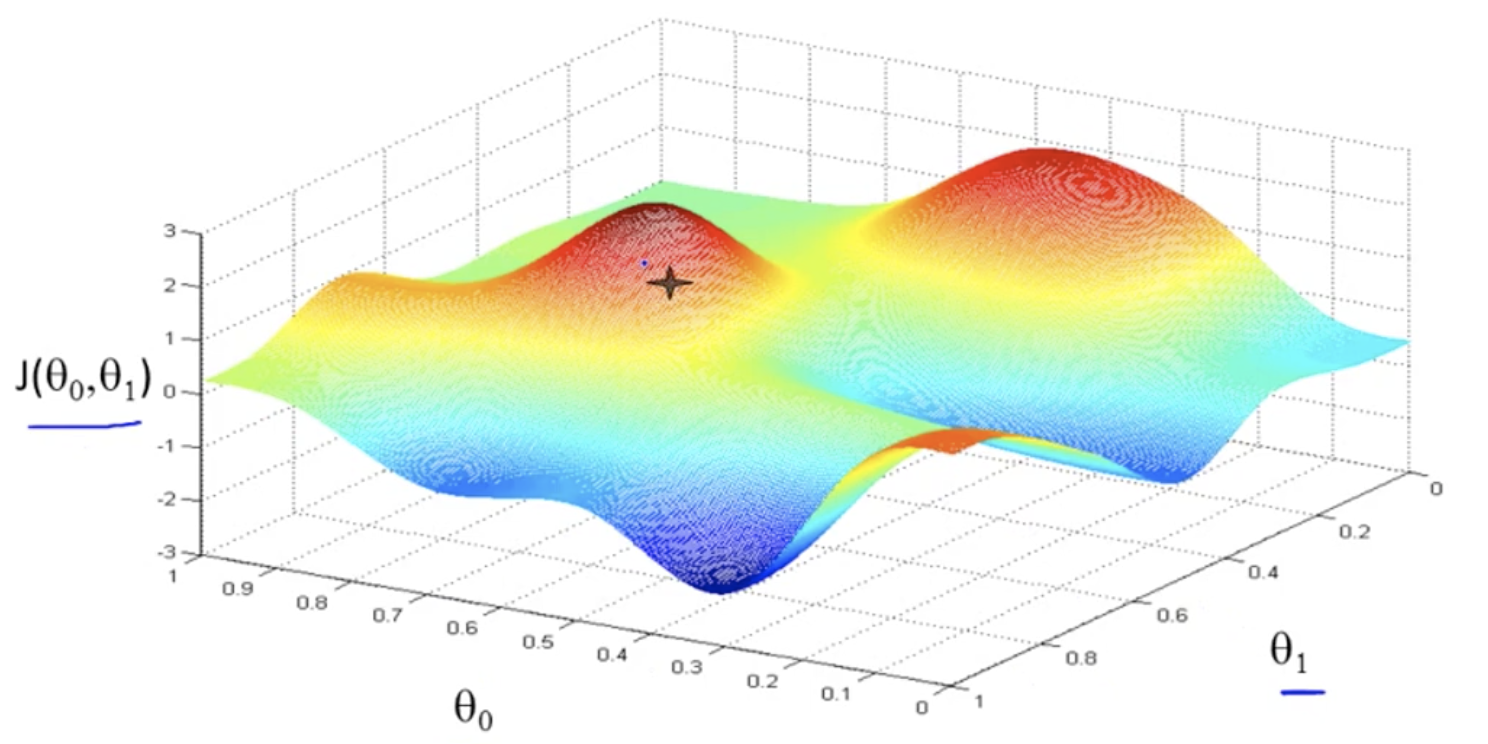
\includegraphics[scale=0.6]{figures/gradient_descent}

Wiederholen bis zur Konvergenz:
$$\Theta_{i} := \Theta_{i} - \alpha\frac{\partial}{\partial \Theta_{i}} J(\Theta_{0}, \Theta_{1}) $$

$$ \alpha: Learning Rate $$
$$ i=0, i=1 $$

\subsubsection{GD für Linear Regression}
Model Funktion:
$$h_{\Theta} = \Theta_{0} + \Theta_{1}x$$
Cost-Function:
$$ J(\Theta_{0}, \Theta_{1}) = \frac{1}{2m} \sum_{i=1}^{m}(h_{\Theta}(x^{(i)})-y^{(i)})^{2} $$

Für lineare Regression hat die Kostenfunktion stets nur ein lokales (sprich globales) Minimum.
\linebreak
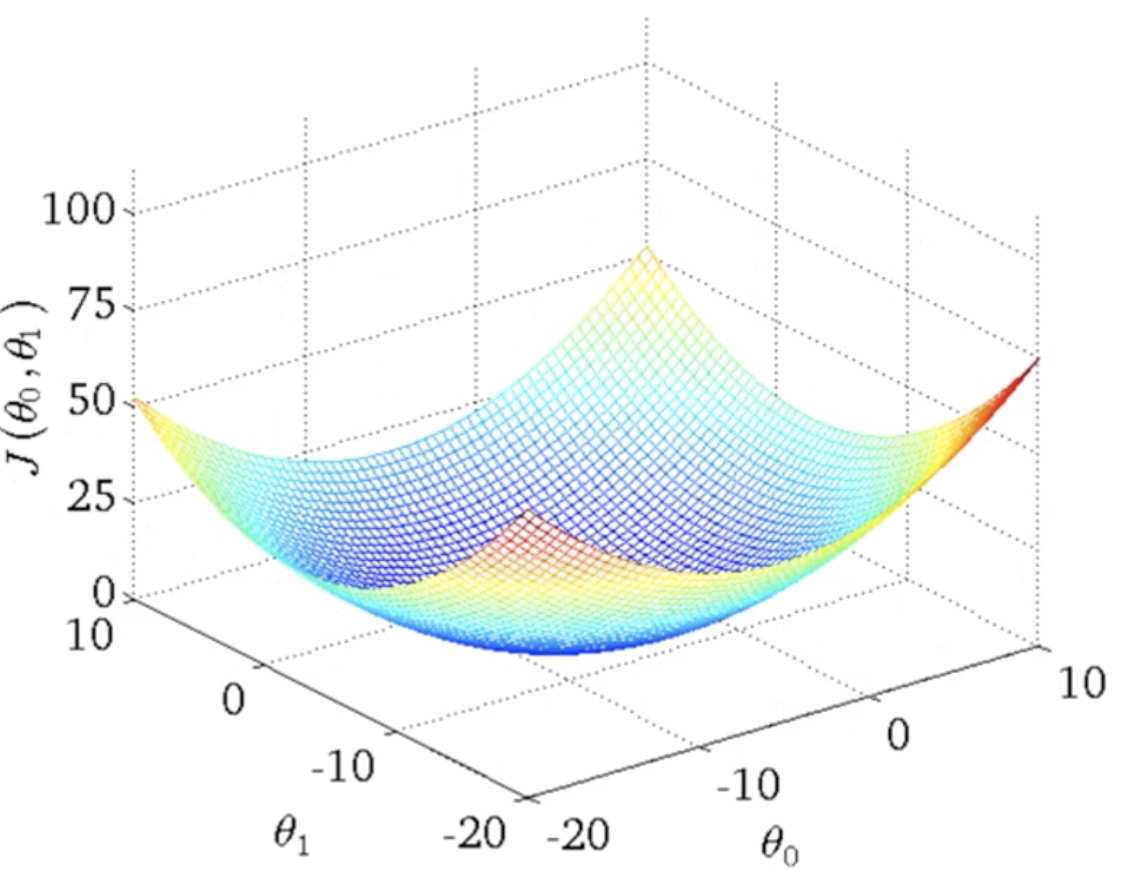
\includegraphics[scale=0.6]{figures/cost_function_linear_regression}
\linebreak
Der Gradient Descent Algorithmus für eine simple Lineare Regression rechnet sich wie folgt:
\linebreak


\begin{algorithm}
\caption{Calculate $\text{min}_{\Theta} J(\Theta)$}
\begin{algorithmic} 
\Repeat 
\State $ \Theta_{0} := \Theta_{0} - \alpha \frac{1}{m} \sum_{i=1}^{m}(h_{\Theta}(x^{(i)}) - y^{(i)}) $

\State $ \Theta_{1} := \Theta_{1} - \alpha \frac{1}{m} \sum_{i=1}^{m}(h_{\Theta}(x^{(i)}) - y^{(i)})*x^{(i)} $
\Comment{simultaneously update all $\Theta_{j}$}
\Until{$J(\Theta_{0}, \Theta_{1})$ converges}
\end{algorithmic}
\end{algorithm}


\end{flushleft}
% ****************************************************************



\newpage
\section{Normal Equation}
\begin{flushleft}

Die Normal Equation ist eine Alternative zum Gradient Descent und rechnet sich wie folgt:

$$ \Theta = (X^{T}X)^{-1}X^{T}y $$

Unterschied zu Gradient Descent:
\begin{table}[h]
	\begin{tabular}{|l|l|}
		\hline
		{\textbf{Gradient Descent}} 		& {\textbf{Normal Equation}} 		\\ \hline
		Alpha muss gewählt werden       & Alpha muss nicht gewählt werden   \\ \hline
		Benötigt viele Iterationen      & Benötigt keine Iterationen        \\ \hline
		$O(kn^{2})$                     & $O(n^{3})$                        \\ \hline
		Auch für grosses n performant   & Langsam für grosses n             \\ \hline
	\end{tabular}
\end{table}
\end{flushleft}

\newpage
\section{Linear Regression}
\begin{flushleft}

Die lineare Regression ist ein Verfahren welches versucht, eine abhängige Variable durch eine oder mehrere unabhängige Variablen zu erklären.

\subsection{Simple lineare Regression}

Die simple lineare Regression arbeitet lediglich im zweidimensionalen Raum.

\begin{tikzpicture}
\begin{axis} [
	axis lines = left, % Only displays axis on left and bottom (not whole box)
	ymin = 0,	% y-axis shall always start at zero
	xlabel = $x$,
	ylabel = $f(x)$,
	mark=*,
	scatter/classes={%	Defines the point appearance for the scatter plot
		a={blue}%,
		%b={mark=triangle*,red},
		%c={mark=o,draw=black}
		}
	]

\addplot [
	domain = 0:60, 	% Range for the value x
	samples = 100,	% Determines the number of points in the interval defined by domain. 
	color = red,	% Color of the
	] {0.83*x + 10.44};
\addlegendentry {$mx + q$}

\addplot [only marks, scatter, scatter src=explicit symbolic]
	table [meta=class] {		% meta defines the column to use for the class of the point
		x		y		class
		10		20		a
		10		15		a
		15		17		a
		20		21		a
		20		31		a
		25		40		a
		30		27		a
		35		40		a
		30		55		a
		40		45		a
		40		37		a
		45		52		a
		50		55		a
		50		45		a
		55		50		a
		60		65		a
		
	};

\end{axis}
\end{tikzpicture}

Die Steigung [m] sowie der y-Achsenabschnitt [q] lassen sich wie folgt berechnen:

$$m = \dfrac{\sum_{i=1}^n (x_{i} - \bar{x})(y_{i} - \bar{y})}
                       {\sum_{i=1}^n (x_{i} - \bar{x})^{2}}$$

$$q = \bar{y} - m\bar{x}$$

Wobei die werte $\bar{x}$, $\bar{y}$ den arithmetischen Mitteln der Definitions- und Bildmenge entsprechen.
\linebreak
Die Qualität eines Regressionsmodells kann durch Genauigkeitsmetriken bestimmt werden. Hierbei werden stets die effektiven Y-Werte mit den jeweiligen Werten $\hat{y}_{i} = mx_{i} + q$ der linearen Regressionslinie verglichen.


Der \textbf{Mittlerer absoluter Fehler} (mean-absolute-error) ist die simpleste Metrik und zeig den effektiven Durchschnittsfehelr auf. 
$$MAE = \dfrac{1}{n}\sum_{i=1}^n|y_{i} - \hat{y}_{i}|$$


Die \textbf{Mittlere quadratische Abweichung} (mean-square-error) reagiert aufgrund des Exponenten proportional stärker auf grosse Fehler.
$$MSE = \dfrac{1}{n}\sum_{i=1}^n(y_{i} - \hat{y}_{i})^{2}$$

Der \textbf{root-mean-square-error} ist die gängigste Metrik, da dieser, durch das Ziehen der Wurzel, in der gleichen Einheit interpretierbar ist wie die eigentlichen Y-Vektoren.
$$RMSE = \sqrt{\dfrac{1}{n}\sum_{i=1}^n(y_{i} - \hat{y}_{i})^{2}} = \sqrt{MSE}$$


\subsection{Polynomial Regression}
\subsection{Multivariable Regression}

\end{flushleft}
\newpage
\section{Logistic Regression Basics}
\label{sec:logistic_regression_basics}

Dieses Kapitel beschreibt die fundamentalen Aspekte (prüfungsrelevanter Teil) der logistischen Regression. Die logistic regression ist ein linearer suppervised Klassifikationsalgorithmus. Genauer genommen einen \textbf{binären} Klassifikationsalgorithmus. \\


\subsection{Logistic Regression vs Adaline}

Die grundlegende Architektur von logistic regression ist sehr ähnlich wie bei Adaline. Der \textbf{Hauptunterschied} liegt bei der Aktivierungsfunktion. Die logistic regression verwendet die sogenannte \textbf{Sigmoid} Funktion.

Für Adaline haben wir lediglich die Identitätsfunktion verwendet.


\begin{figure}[h!]
	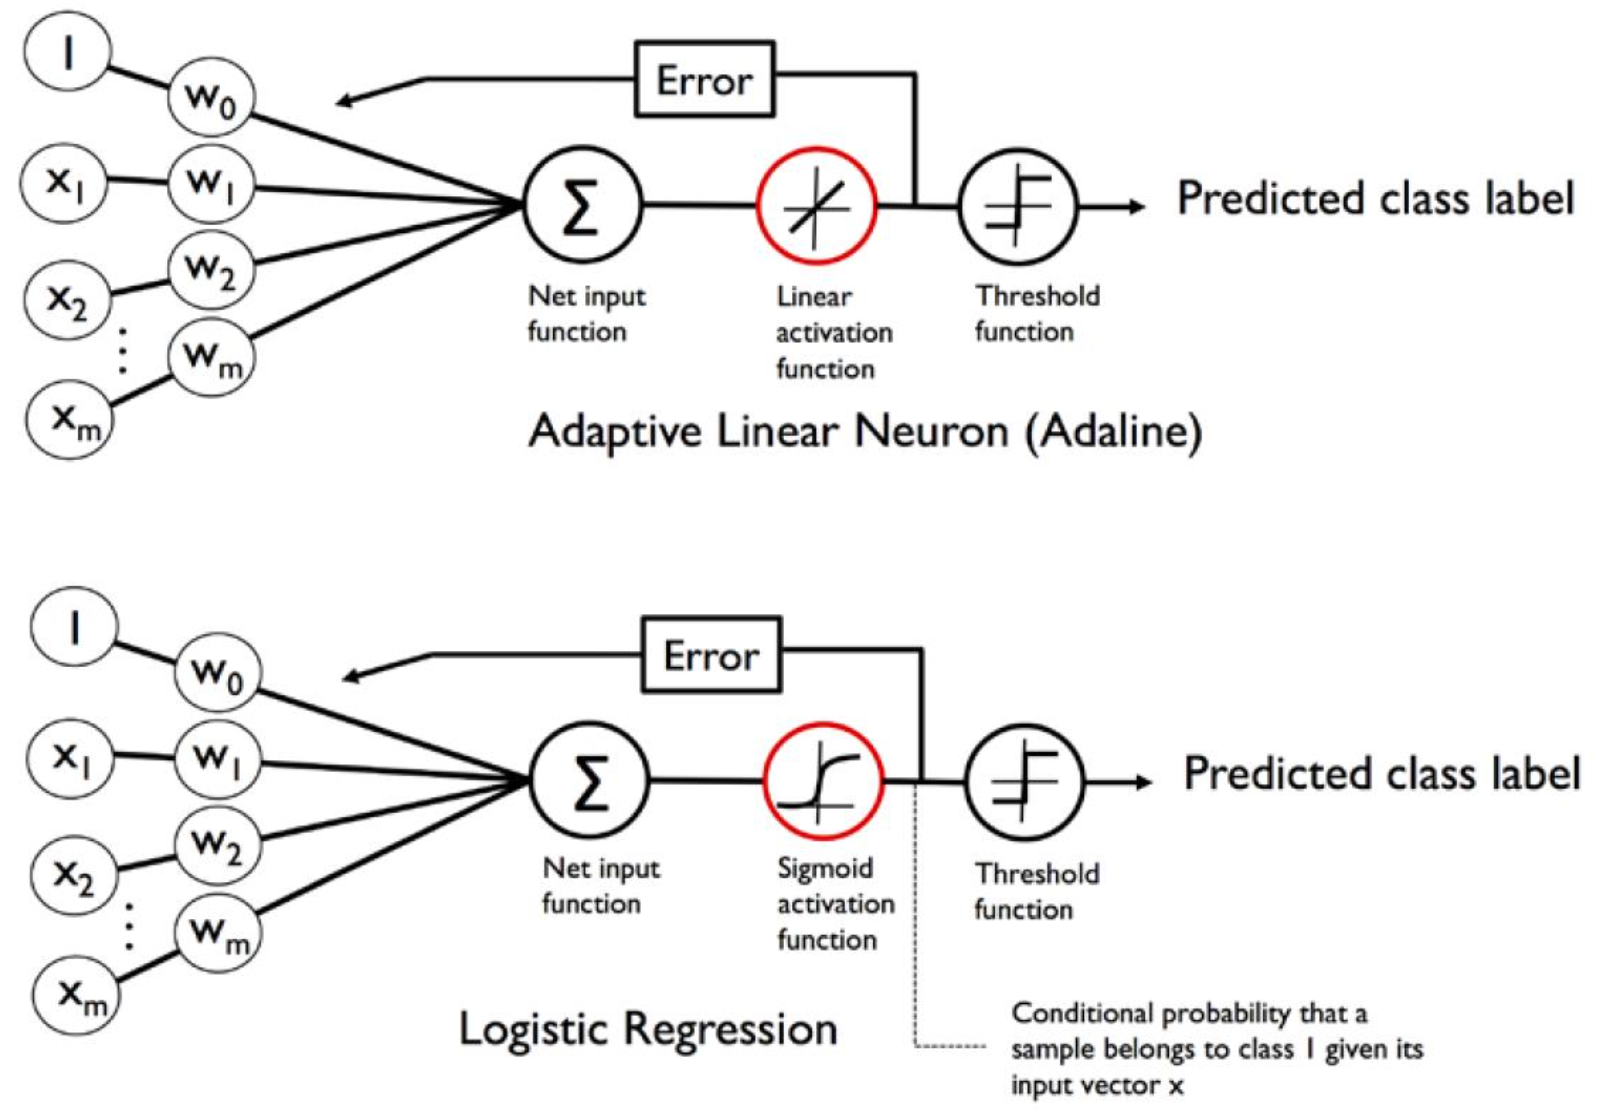
\includegraphics[scale=0.5]{figures/logistic_regression_vs_adaline}
	\caption{Logistic Regression vs Adaline}
	\label{fig:lr_vs_adaline}
\end{figure}


\newpage
\subsection{Sigmoid Funktion}

Die Sigmoid Funktion nimmt einen Input und transformiert diesen in ein Bereich [0,1].

\begin{tikzpicture}[declare function={sigma(\x)=1/(1+exp(-\x));}]
\begin{axis}%
[
    grid=major,     
    xmin=-8,
    xmax=8,
    axis x line=bottom,
    ytick={0,.5,1},
    ymax=1,
    axis y line=middle,
    samples=100,
    domain=-8:8,
    legend style={at={(1,0.9)}}     
]
    \addplot[blue,mark=none]   (x,{sigma(x)});
    \legend{$g(x)$}
\end{axis}
\end{tikzpicture}


$$ \phi(z) = \frac{1}{1 + e^{-z}} $$

Der Wert von $\phi(z)$ kann auch als \textbf{Wahrscheinlichkeit} interpretiert werden, das ein gewisses Sample zu einer bestimmten Klasse gehört.


$$ \phi(z) = \frac{1}{1 + e^{-z}} = P(y=1 | x;w) $$
Hierbei steht $y=1$ für die binäre Klasse 1.
Somit gilt auch der Zusammenhang zur anderen Klasse 0:
$$ P(y=0|x;w) = 1 - P(y=1|x;w)$$


\subsection{Vorteile logistic regression}

\begin{itemize}
	\item Output der Sigmoid kann als Wahrscheinlichkeit interpretiert werden. Dies gibt uns Informationen über die \textbf{Gewissheit} des Models.
	\item Da logistic regression ein \textbf{lineares Model} ist, ist es einfach zu interpretieren, updaten und ist skalierbar.
\end{itemize}

Diese Vorteile machen die logistische Regression zu einer zuverlässige und sinnvolle Wahl für viele Klassifizierungsprobleme.





\newpage
\section{Logistic Regression}
\subsection{Binary classification}
\begin{flushleft}


Mittels Logistischer Regression lassen sich diskrete Phänomene klassifizieren. Die Funktion des Models ist wie folgt definiert:


$$ h_{\Theta}(x) = g(\Theta^{T}x) $$ 
x ist hierbei lediglich der Featurevektor eines Samples $\icol{x_{1}\\x_{2}\\x_{3}}$. Eine vektorielle Implementation für alle Featuresamples (Matrix) ist weiter unten beschrieben.
$$ g(z) = \frac{1}{1 + e^{-z}} $$
$$ h_{\Theta}(x) = \frac{1}{1 + e^{-\Theta^{T}x}} $$

Die Funktion $g(x)$ ist hierbei die sogenannte Sigmoid (oder auch logistische) Funktion.

\begin{tikzpicture}[declare function={sigma(\x)=1/(1+exp(-\x));}]
\begin{axis}%
[
    grid=major,     
    xmin=-8,
    xmax=8,
    axis x line=bottom,
    ytick={0,.5,1},
    ymax=1,
    axis y line=middle,
    samples=100,
    domain=-8:8,
    legend style={at={(1,0.9)}}     
]
    \addplot[blue,mark=none]   (x,{sigma(x)});
    \legend{$g(x)$}
\end{axis}
\end{tikzpicture}

Der Wert $h_{\Theta}(x)$ wird als Wahrscheinlichkeit verstanden, dass der Output (y) positive ist für ein gegebener Eingabewert (x) parametrisiert mit $\Theta$.
\linebreak

Formal definiert:
$$h_{\Theta}(x) = P(y=1|x;\Theta)$$
Somit gilt:
$$ P(y=0|x;\Theta) = 1 - P(y=1|x;\Theta)$$



Cost-Function:

$$ J(\Theta) = \frac{1}{m}\sum_{i=1}^{m}Cost(h_{\Theta}(x^{(i)}), y^{(i)}) $$


$$ \text{Cost}(h_{\Theta}(x), y) =
    \begin{cases}
      -\text{log}(h_{\Theta}(x)) & \text{for } y=1\\
      -\text{log}(1 - h_{\Theta}(x)) & \text{for } y=0\\
    \end{cases} $$

Im Gegensatz zur linearen Regression wird bei der logistischen die Cost-Funktion je nach Fall (Wert von y) unterschieden, um eine konvexe Funktion zu generieren.
Graphisch dargestellt sieht die Cost-Function wie folgt aus:

\begin{tikzpicture}[declare function={c1(\x)=-log2(x); c0(\x)=-log2(1-x);}]
\begin{axis}%
[
    grid=major,     
    xmin=-0.1,
    xmax=1,
    axis x line=bottom,
    ytick={0,1,2,3,4,5},
    ymax=5,
    axis y line=middle,
    samples=1000,
    domain=0:1,
    legend style={at={(1,0.9)}}     
]
    \addplot[blue,mark=none]   (x,{c1(x)});
    \addplot[red,]   (x,{c0(x)});
    \legend{$\text{cost1}(x)$, $\text{cost0}(x)$}
\end{axis}
\end{tikzpicture}


\begin{algorithm}
\caption{Calculate $\text{min}_{\Theta} J(\Theta)$}
\begin{algorithmic} 
\REPEAT 
\STATE $ \Theta_{j} := \Theta_{j} - \alpha\sum_{i=1}^{m}(h_{\Theta}(x^{(i)}) - y^{(i)})x_{j}^{(i)} $
\COMMENT{simultaneously update all $\Theta_{j}$}
\UNTIL{$J(\Theta)$ converges}
\end{algorithmic}
\end{algorithm}

Eine Vektor-Implementation dieses Algorithmus sieht so aus:

$$ \Theta := \Theta - \frac{\alpha}{m} X^{T}(g(X\Theta) - \vec{y}) $$

\subsubsection{Regularization}

TODO


% ****************************************
\subsection{Multiclass classification}
\subsubsection{One-vs-all}

Sei $y = {0, 1, ..., n}$ die zu klassifizierenden Klassen. So wird für jede Klasse in y eine logarithmische Regression gebildet. Die entstehende Funktion unterscheidet zwischen der gerade betrachteten Klasse (i) und allen anderen. Daher wird diese Methode auch One-vs-rest genannt.

$$ y \in {0, 1, ..., n} $$

$$ h_{\Theta}^{(0)}(x) = P(y=0|x;\Theta) $$
$$ h_{\Theta}^{(1)}(x) = P(y=1|x;\Theta) $$
$$ \text{...} $$
$$ h_{\Theta}^{(n)}(x) = P(y=n|x;\Theta) $$

$$ \text{prediction} = \text{max}_{i}(h_{\Theta}^{(i)}(x)) $$








\end{flushleft}





\newpage
\section{Neuronale Netzwerke}
\subsection{Representation}
\begin{flushleft}


Der Inputnode $x_{0}$ wird nicht immer eingezeichnet und repräsentiert den Bias-Node.

Weiter gilt:

$\begin{aligned}
 \alpha_{i}^{(j)} &= \text{Aktivierung der Einheit i im Layer j}
\end{aligned}$

$\begin{aligned}
 \Theta^{(j)} &= \text{Gewichtsmatrix welche Layer j auf Layer j+1 mapt}
\end{aligned}$

\begin{tikzpicture}[
     % define styles 
     clear/.style={ 
         draw=none,
         fill=none
     },
     net/.style={
         matrix of nodes,
         nodes={ draw, circle, inner sep=10pt },
         nodes in empty cells,
         column sep=2cm,
         row sep=-9pt
     },
     >=latex
]
% define matrix mat to hold nodes
% using net as default style for cells
\matrix[net] (mat)
{
% Define layer headings
|[clear]| \parbox{1.3cm}{\centering Input\\layer} 
    & |[clear]| \parbox{1.3cm}{\centering Hidden\\layer} 
    & |[clear]| \parbox{1.3cm}{\centering Output\\layer} \\
         
$x_{0}$  & |[clear]|        & |[clear]| \\
|[clear]|         & $\alpha_{1}^{(2)}$ & |[clear]| \\
$x_{1}$  & |[clear]|        & |[clear]| \\
|[clear]|         & |[clear]|        & |[clear]| \phantom{$a_{0}^{0}$} \\
$x_{2}$  & $\alpha_{2}^{(2)}$ & $$ \\
|[clear]|         & |[clear]|        & |[clear]|  \phantom{$a_{0}^{0}$} \\
$x_{3}$  & |[clear]|        & |[clear]| \\
|[clear]|         & $\alpha_{3}^{(2)}$ & |[clear]| \\
$x_{4}$  & |[clear]|        & |[clear]| \\ 
};
% left most lines into input layers
\foreach \ai in {2,4,6,8,10}
    \draw[<-] (mat-\ai-1) -- +(-2cm,0);
% lines from a_{i}^{0} to each a_{j}^{1}
\foreach \ai in {2,4,6,8,10} {
    \foreach \aii in {3,6,9}
        \draw[->] (mat-\ai-1) -- (mat-\aii-2);
        }
% lines from a_{i}^{1} to a_{0}^{2}
\foreach \ai in {3,6,9}
  \draw[->] (mat-\ai-2) -- (mat-6-3);
    
% right most line with Output label
\draw[->] (mat-6-3) -- node[above] {$h_{\Theta}(x)$} +(2cm,0);
\end{tikzpicture}




$$ \alpha_{1}^{(2)} = g(\Theta_{10}^{(1)}x_{0} +  \Theta_{11}^{(1)}x_{1} + \Theta_{12}^{(1)}x_{2} +\Theta_{13}^{(1)}x_{3} + \Theta_{14}^{(1)}x_{4})$$

$$ \alpha_{2}^{(2)} = g(\Theta_{20}^{(1)}x_{0} +  \Theta_{21}^{(1)}x_{1} + \Theta_{22}^{(1)}x_{2} +\Theta_{23}^{(1)}x_{3} + \Theta_{24}^{(1)}x_{4})$$

$$ \alpha_{3}^{(2)} = g(\Theta_{30}^{(1)}x_{0} +  \Theta_{31}^{(1)}x_{1} + \Theta_{32}^{(1)}x_{2} +\Theta_{33}^{(1)}x_{3} + \Theta_{34}^{(1)}x_{4})$$


$$ h_{\Theta}(x) = \alpha_{1}^{(3)} = g(\Theta_{10}^{(2)}\alpha_{0}^{(2)} + \Theta_{11}^{(2)}\alpha_{1}^{(2)} + \Theta_{12}^{(2)}\alpha_{2}^{(2)} + \Theta_{13}^{(2)}\alpha_{3}^{(2)}) $$


Existiert ein neuronales Netz mit $s_{j}$ Einheiten im Layer $j$, $s_{j+1}$ Einheiten im Layer $j+1$, dann hat $\Theta^{(j)}$ die Dimension $s_{j+1} \times (s_{j} + 1)$.

\end{flushleft}


\subsection{Logik Beispiel}

\subsubsection{AND}
\begin{flushleft}


Ein AND-Gatter kann wie folgt erstellt werden:

\begin{tikzpicture}[
     % define styles 
     clear/.style={ 
         draw=none,
         fill=none
     },
     net/.style={
         matrix of nodes,
         nodes={ draw, circle, inner sep=10pt },
         nodes in empty cells,
         column sep=2cm,
         row sep=-9pt
     },
     >=latex
]
% define matrix mat to hold nodes
% using net as default style for cells
\matrix[net] (mat)
{
% Define layer headings
|[clear]| \parbox{1.3cm}{\centering Input\\layer} & |[clear]| \parbox{1.3cm}{\centering Output\\layer} \\
         
$+1$  		& |[clear]| \\
|[clear]| 	& |[clear]| \\
$x_{1}$  	& |[clear]| \\
|[clear]| 	& $$ \\
$x_{2}$  	& |[clear]| \\
};
\draw[->] (mat-2-1) -- node[above=1mm] {-30} (mat-5-2);
\draw[->] (mat-4-1) -- node[above=1mm] {20} (mat-5-2);
\draw[->] (mat-6-1) -- node[above=1mm] {20} (mat-5-2);
\draw[->] (mat-5-2) -- node[above] {$h_{\Theta}(x)$} +(2cm,0);
\end{tikzpicture}

$$ h_{\Theta}(x) = g(-30 + 20x_{1} + 20x_{2}) $$


\begin{center}
\begin{tabular}{ c c|r } 

 $x_{1}$ & $x_{2}$ & $h_{\Theta}(x)$ \\ 
  \hline
 0 & 0 & $g(-30) \approx 0$ \\ 
 0 & 1 & $g(-10) \approx 0$ \\ 
 1 & 0 & $g(-10) \approx 0$ \\ 
 1 & 1 & $g(10) \approx 1$ \\ 

\end{tabular}
\end{center}
\end{flushleft}


\subsubsection{OR}
\begin{flushleft}


Ein OR-Gatter kann wie folgt erstellt werden:

\begin{tikzpicture}[
     % define styles 
     clear/.style={ 
         draw=none,
         fill=none
     },
     net/.style={
         matrix of nodes,
         nodes={ draw, circle, inner sep=10pt },
         nodes in empty cells,
         column sep=2cm,
         row sep=-9pt
     },
     >=latex
]
% define matrix mat to hold nodes
% using net as default style for cells
\matrix[net] (mat)
{
% Define layer headings
|[clear]| \parbox{1.3cm}{\centering Input\\layer} & |[clear]| \parbox{1.3cm}{\centering Output\\layer} \\
         
$+1$  		& |[clear]| \\
|[clear]| 	& |[clear]| \\
$x_{1}$  	& |[clear]| \\
|[clear]| 	& $$ \\
$x_{2}$  	& |[clear]| \\
};
\draw[->] (mat-2-1) -- node[above=1mm] {-10} (mat-5-2);
\draw[->] (mat-4-1) -- node[above=1mm] {20} (mat-5-2);
\draw[->] (mat-6-1) -- node[above=1mm] {20} (mat-5-2);
\draw[->] (mat-5-2) -- node[above] {$h_{\Theta}(x)$} +(2cm,0);
\end{tikzpicture}

$$ h_{\Theta}(x) = g(-10 + 20x_{1} + 20x_{2}) $$


\begin{center}
\begin{tabular}{ c c|r } 

 $x_{1}$ & $x_{2}$ & $h_{\Theta}(x)$ \\ 
  \hline
 0 & 0 & $g(-10) \approx 0$ \\ 
 0 & 1 & $g(10) \approx 1$ \\ 
 1 & 0 & $g(10) \approx 1$ \\ 
 1 & 1 & $g(30) \approx 1$ \\ 

\end{tabular}
\end{center}
\end{flushleft}


\subsubsection{NOT}
\begin{flushleft}


Ein NOT-Gatter kann wie folgt erstellt werden:

\begin{tikzpicture}[
     % define styles 
     clear/.style={ 
         draw=none,
         fill=none
     },
     net/.style={
         matrix of nodes,
         nodes={ draw, circle, inner sep=10pt },
         nodes in empty cells,
         column sep=2cm,
         row sep=-9pt
     },
     >=latex
]
% define matrix mat to hold nodes
% using net as default style for cells
\matrix[net] (mat)
{
% Define layer headings
|[clear]| \parbox{1.3cm}{\centering Input\\layer} & |[clear]| \parbox{1.3cm}{\centering Output\\layer} \\
         
$+1$  		& |[clear]| \\
|[clear]| 	& $$ \\
$x_{1}$  	& |[clear]| \\
};
\draw[->] (mat-2-1) -- node[above=1mm] {10} (mat-3-2);
\draw[->] (mat-4-1) -- node[above=1mm] {-20} (mat-3-2);
\draw[->] (mat-3-2) -- node[above] {$h_{\Theta}(x)$} +(2cm,0);
\end{tikzpicture}

$$ h_{\Theta}(x) = g(10 - 20x_{1}) $$


\begin{center}
\begin{tabular}{ c|r } 

 $x_{1}$ & $h_{\Theta}(x)$ \\ 
  \hline
 0 & $g(10) \approx 1$ \\ 
 1 & $g(-10) \approx 0$ \\ 

\end{tabular}
\end{center}
\end{flushleft}



\subsubsection{XNOR}
\begin{flushleft}


Durch Kombinationen von einzelnen NN können komplexere Gatter erstellt werden. Wie bspw. das XNOR Gatter.

\begin{tikzpicture}[
     % define styles 
     clear/.style={ 
         draw=none,
         fill=none
     },
     net/.style={
         matrix of nodes,
         nodes={ draw, circle, inner sep=10pt },
         nodes in empty cells,
         column sep=2cm,
         row sep=-9pt
     },
     >=latex
]
% define matrix mat to hold nodes
% using net as default style for cells
\matrix[net] (mat)
{
% Define layer headings
|[clear]| \parbox{1.3cm}{\centering Input\\layer} 
	& |[clear]| \parbox{1.3cm}{\centering Hidden\\layer} 
	& |[clear]| \parbox{1.3cm}{\centering Output\\layer} \\
         
$+1$  		& $+1$ 					&	|[clear]|\\
|[clear]|	& |[clear]|				&	|[clear]| \\
$x_{1}$  	& $\alpha_{1}^{(2)}$  	&  	$\alpha_{1}^{(3)}$\\
|[clear]|	& |[clear]|				&	|[clear]| \\
$x_{2}$  	& $\alpha_{1}^{(2)}$ 	&  	|[clear]|\\
};
% +1
\draw[->] (mat-2-1) -- node[above=0mm] {-30} (mat-4-2);
\draw[->] (mat-2-1) -- node[above=0mm] {10} (mat-6-2);
%  x1
\draw[->] (mat-4-1) -- node[below=0mm] {20} (mat-4-2);
\draw[->] (mat-4-1) -- node[above=0mm] {-20} (mat-6-2);
%  x2
\draw[->] (mat-6-1) -- node[below=0mm] {20} (mat-4-2);
\draw[->] (mat-6-1) -- node[below=0mm] {-10} (mat-6-2);

%
\draw[->] (mat-2-2) -- node[above=0mm] {-10} (mat-4-3);
\draw[->] (mat-4-2) -- node[above=0mm] {20} (mat-4-3);
\draw[->] (mat-6-2) -- node[above=0mm] {20} (mat-4-3);

\draw[->] (mat-4-3) -- node[above] {$h_{\Theta}(x)$} +(2cm,0);

\end{tikzpicture}


\begin{center}
\begin{tabular}{ c c|c c|r } 

 $x_{1}$ & $x_{2}$ & $\alpha_{1}^{(2)}$ & $\alpha_{2}^{(2)}$ & $h_{\Theta}(x)$ \\ 
  \hline
 0 & 0 & 0 & 1 & 1 \\ 
 0 & 1 & 0 & 0 & 0 \\ 
 1 & 0 & 0 & 0 & 0 \\ 
 1 & 1 & 1 & 0 & 1 \\ 

\end{tabular}
\end{center}
\end{flushleft}





% ============================================================



% ============================================================


%\newpage
\section{Tryout}\label{sec:tryout}

\begin{figure}[H]	% H stands for here (place right here)
	\centering
	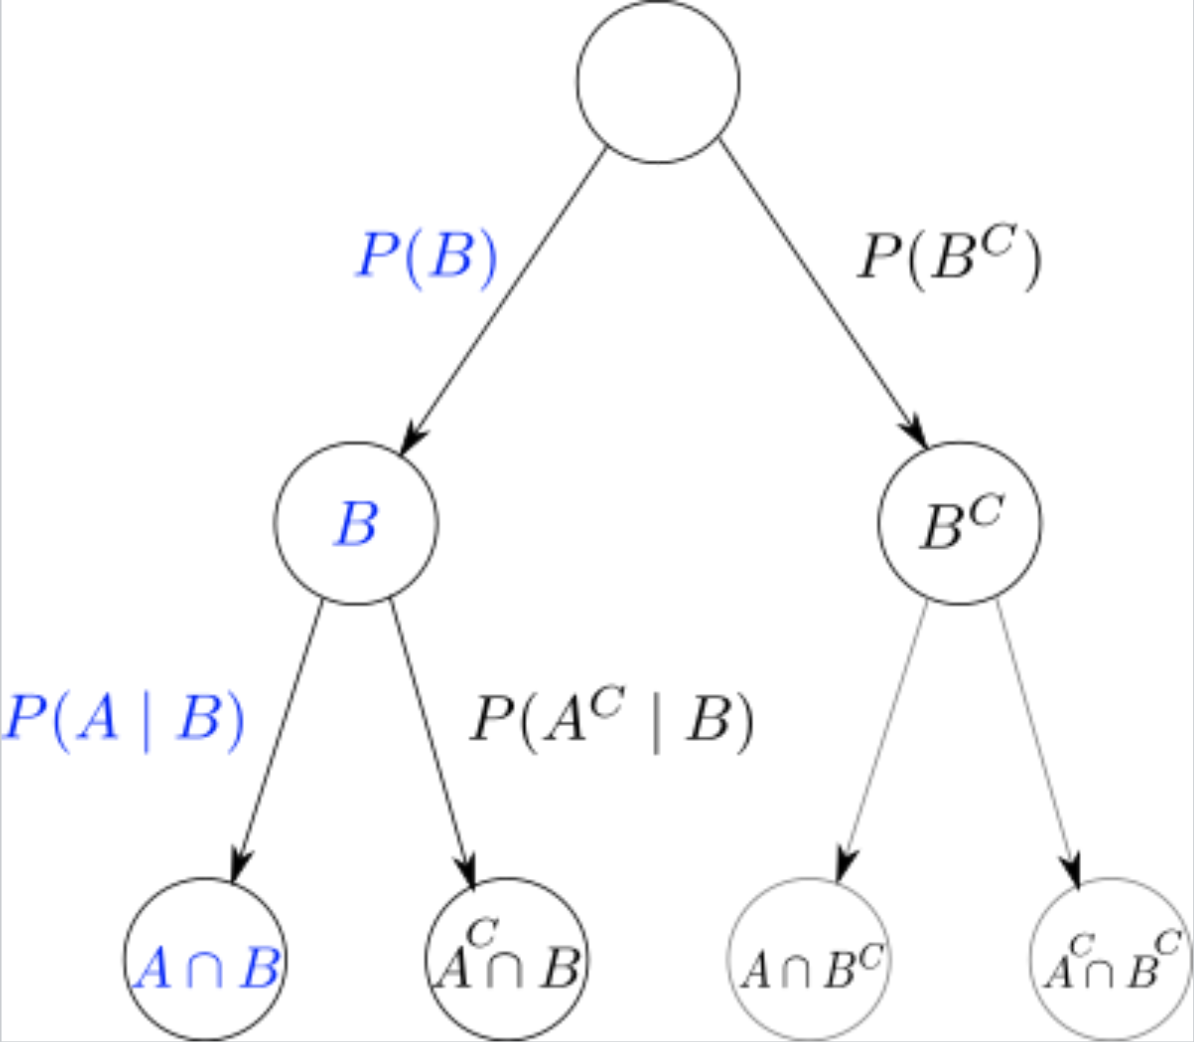
\includegraphics[height=5cm]{figures/tryout.png}
	\caption[Optional optional]{Entscheidungsbaum}
	\label{fig:tryout}
\end{figure}

Wie auf der Abbildung \ref{fig:tryout} zu sehen ist.....


\begin{table}[H]
	\centering
	\label{tab:tryouttab}
\caption[This is an optional caption, without reference]{Local caption, with reference}
	\cite{ref:ds_1, ref:nn_1, ref:ai_1}	% Used to add cites (zitieren)

	\begin{tabular}{l c r}
		Area & Number of rooms & Price \\ \hline
		80	& 4				& 1680 \\
		100	& 5				& 2300 \\
		50	& 2.5				& 1500 \\

	\end{tabular}
\end{table}


\begin{itemize}
	\item This is an item
	\item This is another item
	\begin{itemize}
		\item This is a further item
		\item [blub] This is an item with a custom bullet point
	\end{itemize}
\end{itemize}

\begin{enumerate}
	\item This is a numbered item
	\item And so on
\end{enumerate}


\newpage
\subsection{Math examples}

Here's an example within a sentence $E =mc^2$.

And here one example $$a=v/t$$ which is centred. \\

$$-\frac{\hbar^2}{2m}\frac{d^2\Psi}{dx^2} = E\Psi$$

Fractions

$$d = v_it + \frac{1}{2} \cdot at^2$$
$$d = v_it + \sfrac{1}{2} \cdot at^2$$


Brackets:
$$\left( \frac{1}{2} \right) \cdot 2 = 1$$	% use \left( ..... \right) to match the brackets to the content
$$\left| -7 \right| = 7$$
$$\sqrt{4} = 2$$
$$\sqrt{4} \ne 1$$
$$\sqrt{4} < 5$$
$$ \pi \approx 3 $$
$$ \pi \times \sqrt{4} < 15 $$

\begin{eqnarray}	% Equation array
	3x + 14 &=& 20 \\
	3x &=& 6 \\
	x &=& 2
\end{eqnarray}

\begin{equation}
\label{eq:first}
x^2 + 3x - 7 = 0
\end{equation}

\newpage
\subsection{Graphs}




\begin{tikzpicture}[sibling distance=12em,
							%root/.style={treenode,circle,draw},
							every child node/.style={circle, draw=black},
							]
%	[align=center, sibling distance=5cm]
	\node[fill=black]{}
		child { node {B}
		[sibling distance=6em]
			child { node{A $\cap$ B}  edge from parent node[left] {$P(A|B)$} }
			child { node{$\bar{A} \cap B$} edge from parent node[right] {$P(\bar{A}|B)$}}
			}
		child{ node{$\bar{B}$}
			[sibling distance=6em]
			child{ node{$A \cap \bar{B}$} edge from parent node[left] {$P(A|\bar{B})$}}
			child{ node{$\bar{A} \cap \bar{B}$} edge from parent node[right] {$P(\bar{A}|\bar{B})$} }
		       }
	;

\end{tikzpicture}
% ****************************************************************

% ============================================================




% REFERENCES ============================================================
\cleardoublepage
%\renewcommand{\bibname}{Referenzen}	% Rename the bibliography title
\bibliographystyle{IEEEtran}	% Adds cites (Zitate)
\addcontentsline{toc}{section}{Referenzen}
% references can easily be generated using the OS X tool "BibDesk"
% Make sure you build your LaTeX document in BibTeX after defining your references
%	in order to make them valid.
\bibliography{references/book_ref1}
% ============================================================

% APPENDIX ============================================================
\cleardoublepage
\appendix
\section{Cheatsheet}
% ============================================================


\end{document}